% !TEX root = ../main.tex

\subsection{Baseline event selection}\label{sec:baseline}
This analysis is developed on top of the SM search for the decay of the Higgs boson into a pair of tau leptons \cite{Sirunyan:2017khh}. Consequently, Higgs boson events are tagged exploiting the same baseline event selection. 
They are identified in four of the in total six combinatorically possible decay channels of the tau leptons. These are the $e\mu$, $e\tau_\text{h}$, $\mu\tau_\text{h}$ and $\tau_\text{h}\tau_\text{h}$ channels.
The $ee$ and $\mu\mu$ channels are disregarded because they have both a small branching fraction and suffer from an overwhelming background of $Z\rightarrow ee/\mu\mu$ events. 
The notation used above refers to events with leptonically decaying tau leptons by the final state lepton that triggers the event. For instance, $\tau_\text{e}$ is denoted $e$ and $\tau_\mu$ is called $\mu$.
The lepton and tau candidates are triggered with the same HLT menus as used in Ref. \cite{Sirunyan:2017khh}. The requirements of the trigger menus and the criteria on the isolation are summarized in \tabreft{ES:tab:channels}. 
Only events with exactly two leptons are considered to make the channels exclusive among each other. This means events with additional loosely identified and isolated leptons are rejected. Moreover, leptons must have opposite-sign electric
charges as they possibly originate from the electrically neutral Higgs boson. Ditau pairs are constructed using the pair matching algorithm from Ref. \cite{Sirunyan:2017khh}. 
Last but not least, requirements on the compatability with the PV of the event are imposed. Therefore, leptons must satisfy d\textunderscript{xy}\,<\,0.045\,{cm} and d\textunderscript z\,<\,0.2\,{cm}. \newline{} 
In the semileptonic decay channels, $e\tau_\text{h}$ and $\mu\tau_\text{h}$, \textit{W+jets} events become a major source of background. These are rejected by requiring the transverse mass to be
\begin{equation}
    m_\text{T} = \sqrt{2p^\ell_\text{T} E_\text{T}^{\text{miss}} \li 1- \cos \li \Delta \phi \re \re} < \text{50\,{GeV}},
\end{equation}
with the transverse momentum of the lepton $p^\ell_\text{T}$ and the angle $\Delta\phi$ between the lepton and the missing transverse energy $E_\text{T}^\text{miss}$. 
The choice of $m_\text{T}< \text{50\,{GeV}}$ was investigated in \cite{Sirunyan:2017khh} and found to provide a close-to-optimal signal acceptance and background rejection.
The distribution of \mt{} for the \textit{0-jet} category \textref{sec:categorization} in the semileptonic channels are shown in \figreft{ES:dzeta}.
% Blinded distributions of the transverse mass 
% HiggsAnalysis/KITHiggsToTauTau/scripts/makePlots_controlPlots.py -i /nfs/dust/cms/user/dwolfsch/htautau/artus/2018-08-07_18-44_Run2CPStudies_Nominal_Summer16_plusHToTauTauM110-140/merged/ -s ztt zll ttj vv wj qcd qqh gghjhusm data -c et mt -x mt_1 --categories ZeroJetCP BoostedCP dijet2D_lowboost dijet2D_boosted -a "  --live --mask-histogram-nicks data ratio_Data --mask-below-threshold 50  --formats png pdf --y-subplot-lims 0.7 1.3"  --background-method simeqn --cpggh --www EventSelection/control_plots/ -r --analysis-modules MaskHistograms -n 8

\begin{table}[h]
    \centering
    \caption[Baseline selection of lepton pairs.]{Minimum selection criteria for the lepton pairs. The requirements are slightly tighter than actually imposed in the HLT menus to reduce the impact originating from the turn-on curve of the trigger. In the $e\mu$ and $\mu\tau_\text{h}$ channels several triggers are used. The setups used for these different triggers are highlighted accordingly. Adapted from Ref. \cite{Sirunyan:2017khh}.}\label{ES:tab:channels}
    \begin{tabular}{lllll}
        \toprule
        Channel                       & \multicolumn{3}{c}{Selection criteria}                       \\ \cline{2-4}
                                      & $p_\text{\,T} / \text{GeV}$                    & $\eta$                              & Isolation \\ \midrule
\multirow{4}{*}{$e\mu$}               & \cellcolor{ctcolormain!20}{$p_\text{\,T}^e > \text{13}$  }                 & \cellcolor{ctcolormain!20}{$\abs{\eta^e}<\text{2.5}$    }              & \multirow{2}{*}{$I^e < \text{0.15}$} \\
                                      & \cellcolor{ctcolormain!20}{$p_\text{\,T}^\mu > \text{24}$}                 & \cellcolor{ctcolormain!20}{$\abs{\eta^\mu}<\text{2.4}$  }              &                               \\
                                      & \cellcolor{ctcoloraccessory!20}{$p_\text{\,T}^e > \text{24}$      }            & \cellcolor{ctcoloraccessory!20}{$\abs{\eta^e}<\text{2.5}$   }               & \multirow{2}{*}{$I^\mu < \text{0.2}$}   \\
                                      & \cellcolor{ctcoloraccessory!20}{$p_\text{\,T}^\mu > \text{15} $   }            & \cellcolor{ctcoloraccessory!20}{$\abs{\eta^\mu}<\text{2.4}$ }               &                               \\ \midrule
\multirow{2}{*}{$e\tau_\text{h}$}     & $p_\text{\,T}^e > \text{26}$                   & $\abs{\eta^e} < \text{2.1}$                  & $I^e < \text{0.1}$       \\
                                      & $p_\text{\,T}^{\tau_\text{h}} > \text{30}$   & $\abs{\eta^{\tau_\text{h}}}< \text{2.3}$  &  MVA  $\tau_\text{h}$ ID \\  \midrule 
\multirow{4}{*}{$\mu\tau_\text{h}$}   & \cellcolor{ctcolormain!20}{$p_\text{\,T}^\mu > \text{23}$               }  & \cellcolor{ctcolormain!20}{$\abs{\eta^\mu}<\text{2.1}$               } & \multirow{2}{*}{$I^\mu < \text{0.15}$} \\
                                      & \cellcolor{ctcolormain!20}{$p_\text{\,T}^{\tau_\text{h}} > \text{30}$ }  & \cellcolor{ctcolormain!20}{$\abs{\eta^{\tau_\text{h}}}<\text{2.3}$ } &                               \\
                                      & \cellcolor{ctcoloraccessory!20}{$20<p_\text{\,T}^\mu < \text{23}$            }  & \cellcolor{ctcoloraccessory!20}{$\abs{\eta^\mu}<\text{2.1}$              }  & \multirow{2}{*}{MVA  $\tau_\text{h}$ ID}   \\
                                      & \cellcolor{ctcoloraccessory!20}{$p_\text{\,T}^{\tau_\text{h}} > \text{15} $}  & \cellcolor{ctcoloraccessory!20}{$\abs{\eta^{\tau_\text{h}}}<\text{2.3}$}  &                               \\ \midrule  
$\tau_\text{h}\tau_\text{h}$          & $p_\text{\,T}^{\tau_\text{h}}>\text{50 \& 40}$ & $\abs{\eta^{\tau_\text{h}}}<\text{2.1}$  & MVA $\tau_\text{h}$ ID \\ \bottomrule                                
    \end{tabular}%
\end{table}%
\begin{figure}[h!]
    \centering
    \begin{subfigure}{0.45\textwidth}
        \centering
        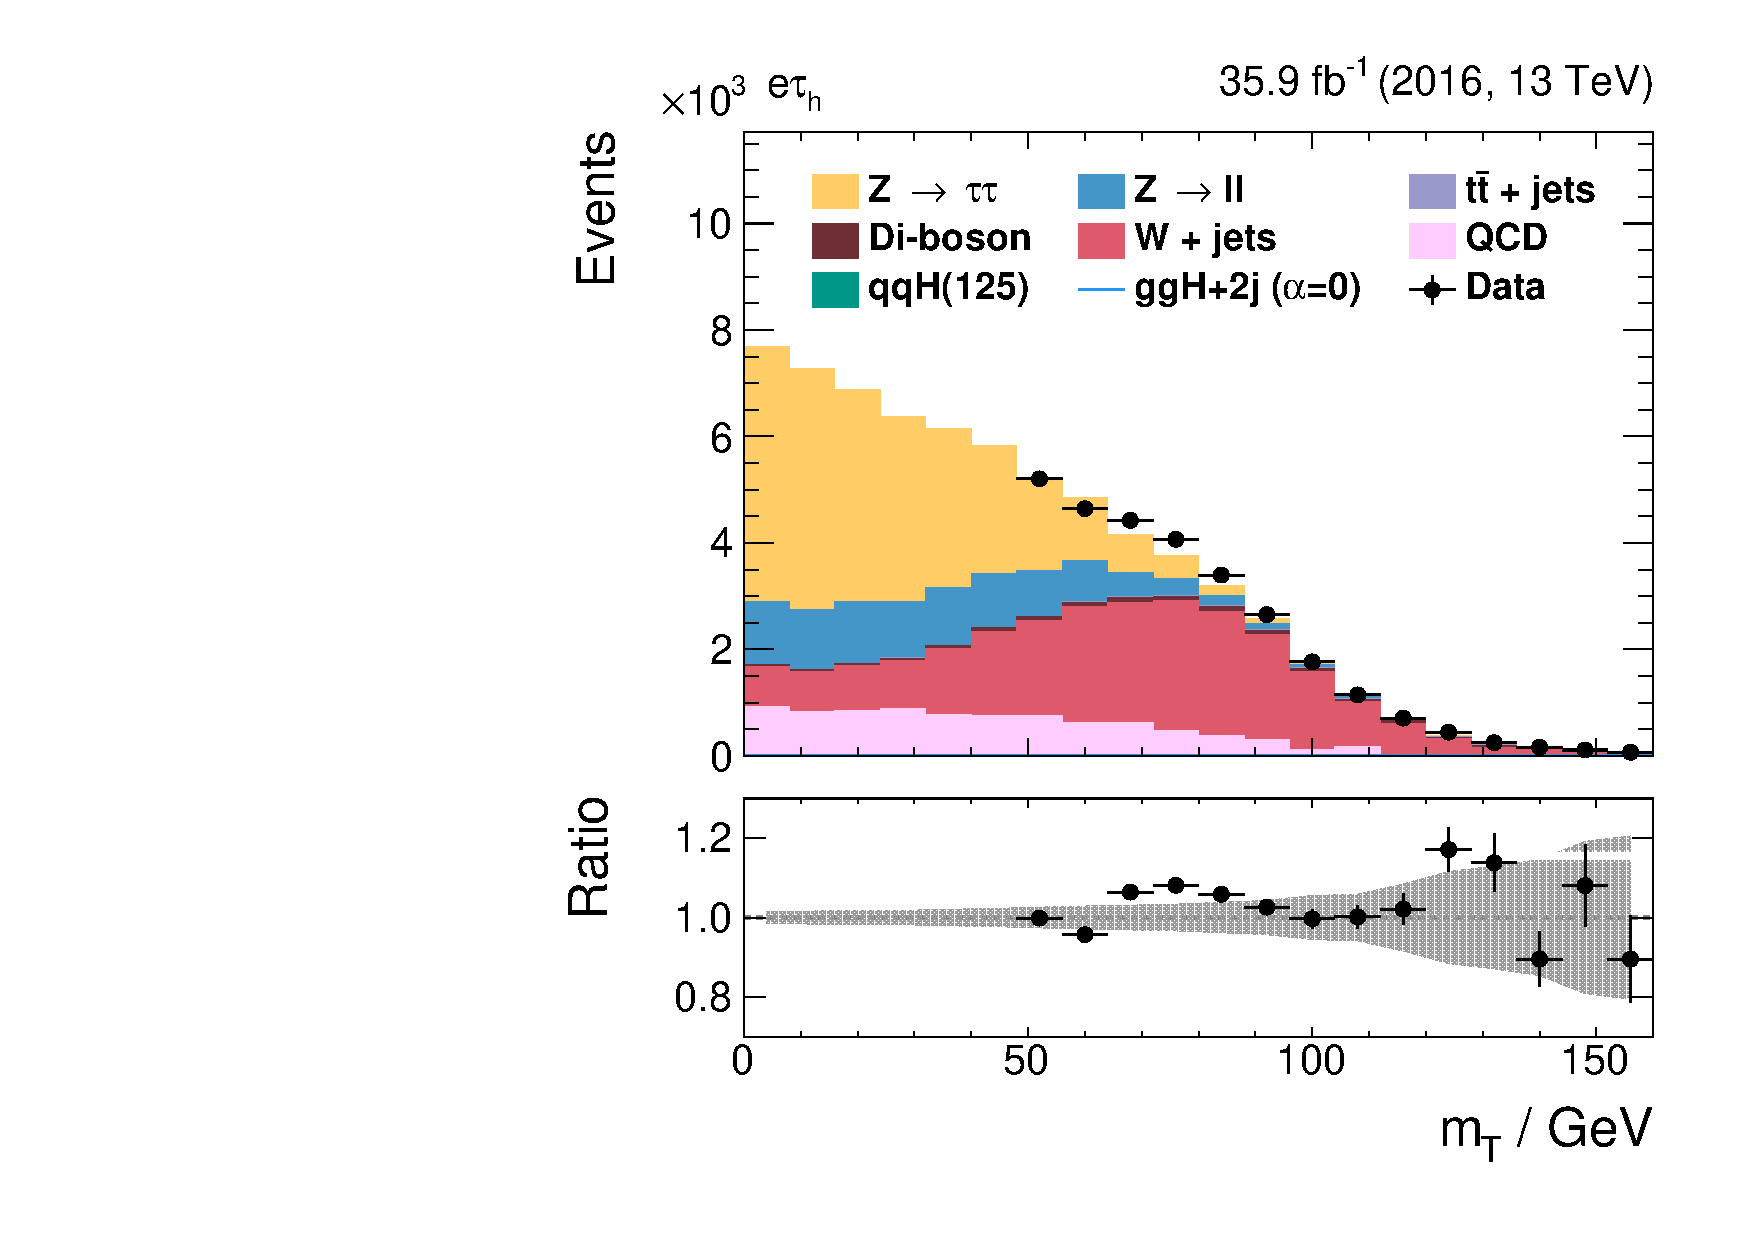
\includegraphics[width=\textwidth]{Figures/eventselection/control_plots/et/ZeroJetCP/mt_1.pdf}%
    \end{subfigure}
    \begin{subfigure}{0.45\textwidth}
        \centering
        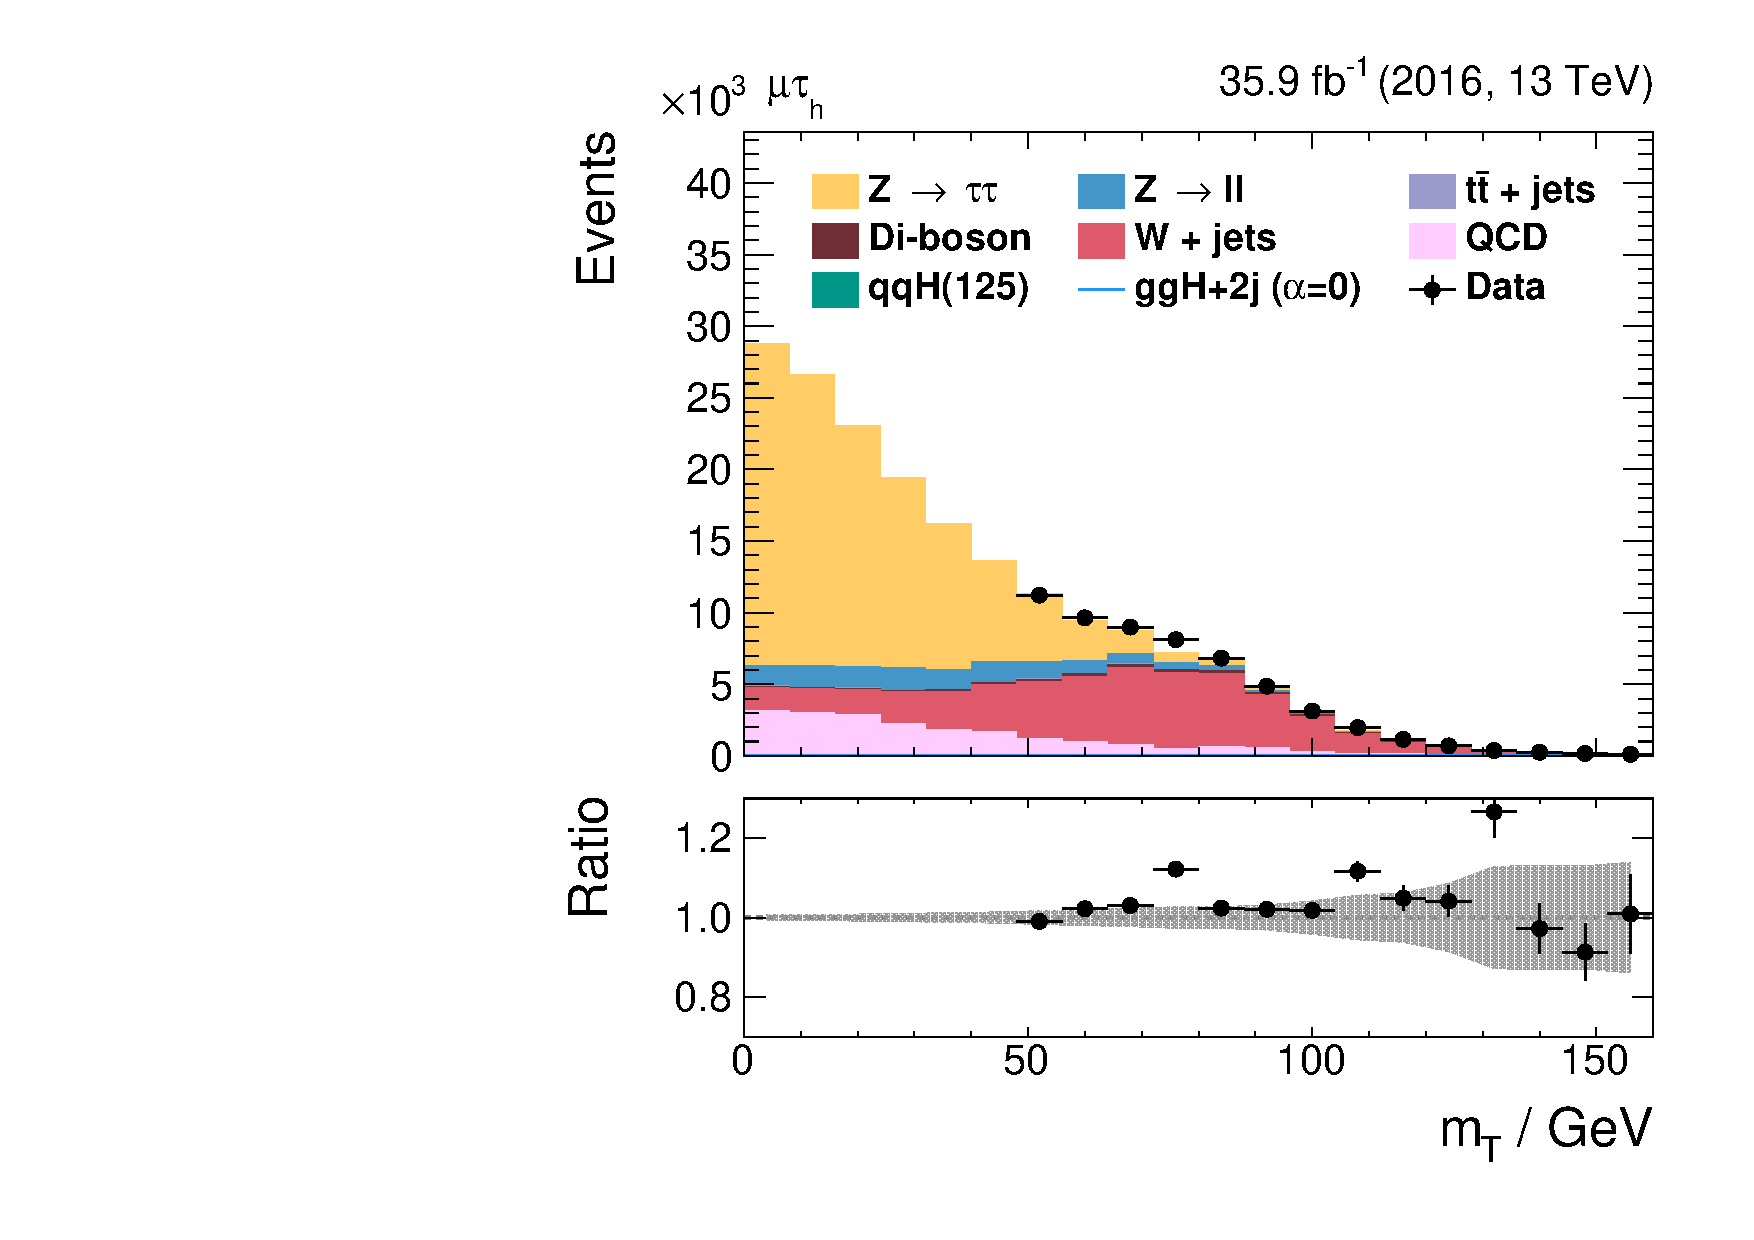
\includegraphics[width=\textwidth]{Figures/eventselection/control_plots/mt/ZeroJetCP/mt_1.pdf}%
    \end{subfigure}        
    \caption[\mt{} control plots in \textit{0-jet} category.]{The transverse mass expected background distribution in the
    \textit{0-jet} category estimated with the techniques introduced in \textreft{sec:background_estimation} and data blinded for $m_\text{T}<\text{50\,{GeV}}$ are shown for the $e\tau_\text{h}$ (left) and $\mu\tau_\text{h}$ (right) channels.}\label{ES:dzeta}%
\end{figure}% 


\clearpage
\subsection{Event kinematics and CP sensitive observables}\label{sec:jdphi}
% - show the event kinematics of a Higgs boson produced in ggF
% - explain the possible angles
% - introduce Deltaphijj as goldplated variable - Why is it sensitive to CP properties?
% - Introduce matrix element techniques - why are they useful? / MELA
% - Introduce the D0- and DCP variables
The different tensor structures in the effective Lagrangian of the scalar and pseudoscalar couplings between the Higgs boson and the gluon fields 
lead to different kinematic distributions of the observable objects in the fermionic couplings in $\mathsf{gg\rightarrow H+2j \rightarrow \tau^+\tau^-+2j}$ events. The production via ggF and decay into tau leptons of a Higgs boson at rest is shown in \figreft{ES:event_kinematics}.
The outgoing particles produced in the event carry information about the quantum numbers and couplings because these quantities must be conserved at each interaction vertex. Generally, information about spin and parity is encoded in angular distributions. 
Consequently, the five angles $\Omega = \{\Delta\phi_\text{jj}, \theta_1, \theta_2, \theta^*,\phi_2 \}$ in the sketch in \figreft{ES:event_kinematics} must contain all this information. The figure shows the kinematic situation of  $\mathsf{gg\rightarrow H+2j \rightarrow \tau^+\tau^-+2j}$ events in the rest frame of the Higgs boson.
The two initial-state jets span up two production planes together with the incoming partons, whose directions are aligned with the directions of the colliding protons. Furthermore, the intersection of the two production planes and the flight direction of the tau leptons span up an additional decay plane. As the tau leptons are produced back-to-back in the
rest frame of the Higgs boson, they do not build a linearly independent set of two vectors necessary to span up a plane by their own.\newline{}
It was found that the signed azimuthal difference between the two initial-state jets $\Delta\phi_\text{jj}$ defined by 
\begin{equation}
    \Delta\phi_\text{jj} = \phi_{\text{j}_1} - \phi_{\text{j}_2 }, \tab \text{with} \, \eta_{\text{j}_1} > \text{0}\, \text{and} \,  \eta_{\text{j}_2} < \text{0}
\end{equation}
already contains much of the total information and is consequently particularly sensitive to the dissimiliarities of scalar and pseudoscalar couplings \cite{Hankele:2006ma,Plehn:2001nj}.
 $\Delta\phi_\text{jj}$ is a signed angle, that is uniquely defined by subtracting the azimuthal angle of the backward jet from the forward jet.
 \begin{figure}[h]
     \centering
     \begin{tikzpicture}[line width=1.5pt]
% https://github.com/thomas-mueller/PhdThesis/tree/master/doc/thesis/figures/latex

\draw[gluon, ctcoloraccessory] (0:0cm) -- (0:2cm);
\node[ctcoloraccessory] at (20:1.5cm) {$g$};
\draw[fermion, ctcoloraccessory] ($ (0:4cm) + (90+10:3cm) $) -- (0:2cm);
\node[ctcoloraccessory] at ($ (0:2cm) + (70:2.75cm) $) {$q$};
\draw[fermion, ctcoloraccessory] (0:2cm) -- ($ (0:4cm) + (90+10+180:3.0cm) $);
\node[ctcoloraccessory] at ($ (0:2cm) + (-58:3cm) $) {$q$};

\draw[gluon, ctcolormain] (180:0cm) -- (180:2cm);
\node[ctcolormain] at (180-20:1.5cm) {$g$};
\draw[gluon, ctcolormain] ($ (180:4cm) + (90-20:3.0cm) $) -- (180:2cm);
\node[ctcolormain] at ($ (180:2cm) + (120:2cm) $) {$g$};
\draw[gluon, ctcolormain] (180:2cm) -- ($ (180:4cm) + (90-20+180:3.0cm) $);
\node[ctcolormain] at ($ (180:2cm) + (-129:3.1cm) $) {$g$};

\fill[black] (0:0cm) circle (0.15cm);
\node[black] at (70:0.55cm) {$H$};

\draw[ctcoloraccessory, dotted, thin] (0:2cm) -- (0:4cm);
\fill[ctcoloraccessory, opacity=0.1] (90+10:3.0cm) -- ($ (0:4cm) + (90+10:3.0cm) $) -- ($ (0:4cm) + (90+10+180:3.0cm) $) -- (90+10+180:3.0cm);
\draw[ctcoloraccessory, -, dashed, very thin] (90+10:3.0cm) -- ($ (0:4cm) + (90+10:3.0cm) $) -- ($ (0:4cm) + (90+10+180:3.0cm) $) -- (90+10+180:3.0cm) -- (90+10:3.0cm);
\fill[ctcoloraccessory] (0:2cm) circle (0.1cm);

\draw[black] (0:2.8cm) arc (0:-50:0.8cm);
\node[black] at ($ (0:2cm) + (-25:1.2cm) $) {$\vartheta_1$};

\draw[ctcolormain, dotted, thin] (180:2cm) -- (180:4cm);
\fill[ctcolormain, opacity=0.1] (90-20:3.0cm) -- ($ (180:4cm) + (90-20:3.0cm) $) -- ($ (180:4cm) + (90-20+180:3.0cm) $) -- (90-20+180:3.0cm);
\draw[ctcolormain, -, dashed, very thin] (90-20:3.0cm) -- ($ (180:4cm) + (90-20:3.0cm) $) -- ($ (180:4cm) + (90-20+180:3.0cm) $) -- (90-20+180:3.0cm) -- (90-20:3.0cm);
\fill[ctcolormain] (180:2cm) circle (0.1cm);

\draw[black] (180:1.4cm) arc (0:-136:0.6cm);
\node[black] at ($ (180:2cm) + (-68:1cm) $) {$\vartheta_2$};

\draw[black] (-80:1.2cm) arc (-80:-110:1.2cm);
\node[black] at (-95:1.6cm) {$\Delta\phi_{jj}$};

\draw[fermion, gray] (90+40:3.0cm) -- (0:0cm);
\node[gray] at (90+40:3.35cm) {$\tau^+$};
\draw[fermion, gray] (0:0cm) -- (90+40+180:3.0cm);
\node[gray] at (90+40+180:3.35cm) {$\tau^-$};
\fill[black] (0:0cm) circle (0.15cm);

\fill[gray, opacity=0.1] ($ (0:4cm) + (90+40:3.0cm) $) -- ($ (0:4cm) + (90+40+180:3.0cm) $) -- ($ (180:4cm) + (90+40+180:3.0cm) $) -- ($ (180:4cm) + (90+40:3.0cm) $);
\draw[gray, -, dashed, very thin] ($ (0:4cm) + (90+40:3.0cm) $) -- ($ (0:4cm) + (90+40+180:3.0cm) $) -- ($ (180:4cm) + (90+40+180:3.0cm) $) -- ($ (180:4cm) + (90+40:3.0cm) $) -- ($ (0:4cm) + (90+40:3.0cm) $);

\draw[black] (0:0.8cm) arc (0:-50:0.8cm);
\node[black] at (-25:1.2cm) {$\vartheta^*$};

\draw[black] ($ (0:4cm) + (-50:1.2cm) $) arc (-50:-80:1.2cm);
\node[black] at ($ (0:4cm) + (-65:1.6cm) $) {$\varphi_2$};

\end{tikzpicture}

     \caption[Event kinematics of $\mathsf{gg\rightarrow H+2j}$ events.]{Production (blue and orange) and decay (grey) planes in the rest frame of a Higgs boson produced via gluon-gluon fusion and decaying into a pair of tau leptons. The incoming partons 
     and the initial-state produced gluons and quarks span up two production planes with azimuthal anglular difference $\Delta\phi_\text{jj}$. A further decay plane
     is defined by the intersection of the two production planes and the direction of the two tau leptons.}\label{ES:event_kinematics}
 \end{figure}%
As indicated in \figreft{ES:event_kinematics} the angle represents the azimuthal separation of the two production planes spanned by the incoming and outgoing partons creating the two 
gluons that produce the Higgs boson. The shape of $\Delta\phi_\text{jj}$ for three different CP hypotheses is shown in \figreft{ES:jdphi_shapes}.
Without any further selection criteria ,all hypotheses have very similar shapes. Using an additional cut of $m_\text{jj}>\text{300\,{GeV}}$ as motivated in Ref. \cite{harris_paper} the shape differences become more pronounced. For scalar couplings the two initial-state jets are emitted parallel or anti-parallel, whereas jets originating from a pseudoscalar interaction are more likely to be orthogonal to each other in the azimuthal plane. 
% As shown in \figreft{ES:mjj} the reason for the better separation is due to the larger kinematical differences in the tail of the distribution. When the distributions are normalized to SM expectation the larger relative difference
% in events with $m_\text{jj}>300\,GeV$ is clearly noticeable. This observation motivates that CP information is more likely to be found in ggF events with a VBF-like topology.
% Commands to produce jdphi shape distributions
% makePlots_controlPlots.py -i /nfs/dust/cms/user/dwolfsch/htautau/artus/2018-08-07_18-44_Run2CPStudies_Nominal_Summer16_plusHToTauTauM110-140/merged/ -s gghjhusm gghjhumm gghjhups -c tt -x jdphi --shapes -a " --colors material_blue2  material_green material_orange -m LINE --x-bins \"16,-3.141,3.141\" --filename JHU_jdphi_no_cuts --live --y-lims 0 0.11 --legend-markers LINE  --formats png pdf --y-lims 0 0.15 "  --www CPHypotheses -w "(njets>1)"
% makePlots_controlPlots.py -i /nfs/dust/cms/user/dwolfsch/htautau/artus/2018-08-07_18-44_Run2CPStudies_Nominal_Summer16_plusHToTauTauM110-140/merged/ -s gghjhusm gghjhumm gghjhups -c tt -x jdphi --shapes -a " --colors material_blue2  material_green material_orange -m LINE --x-bins \"16,-3.141,3.141\" --filename JHU_jdphi_mjj_cuts --live --y-lims 0 0.11 --legend-markers LINE --formats png pdf --y-lims 0 0.15 "  --www CPHypotheses -w "(njets>1)*(mjj>300)"
% mjj distribution and comparison
%  makePlots_controlPlots.py -i /nfs/dust/cms/user/dwolfsch/htautau/artus/2018-08-07_18-44_Run2CPStudies_Nominal_Summer16_plusHToTauTauM110-140/merged/ -s gghjhusm gghjhumm gghjhups -c  tt -x mjj -a " --live --www mjj_signaldistribution --ratio-denominator-nicks gghjhusm125jhusm gghjhusm125jhusm gghjhusm125jhusm --ratio-numerator-nicks gghjhusm125jhusm gghjhumm125jhumm gghjhups125jhups --ratio-result-nicks smsm mmsm pssm --subplot-nicks pssm smsm mmsm --y-subplot-label \"Ratio to SM\"  --stacks 1 2 3 4 5 6 --formats png pdf --y-label "#frac{1}{N}#frac{dN}{dm_\text{jj}}" --y-title-offset 1.1 --legend-cols 1 --legend 0.5 0.5 0.87 0.9  " --analysis-modules NormalizeToUnity Ratio
\begin{figure}[h!]
    \centering
    \begin{subfigure}{.45\textwidth}
        \centering
        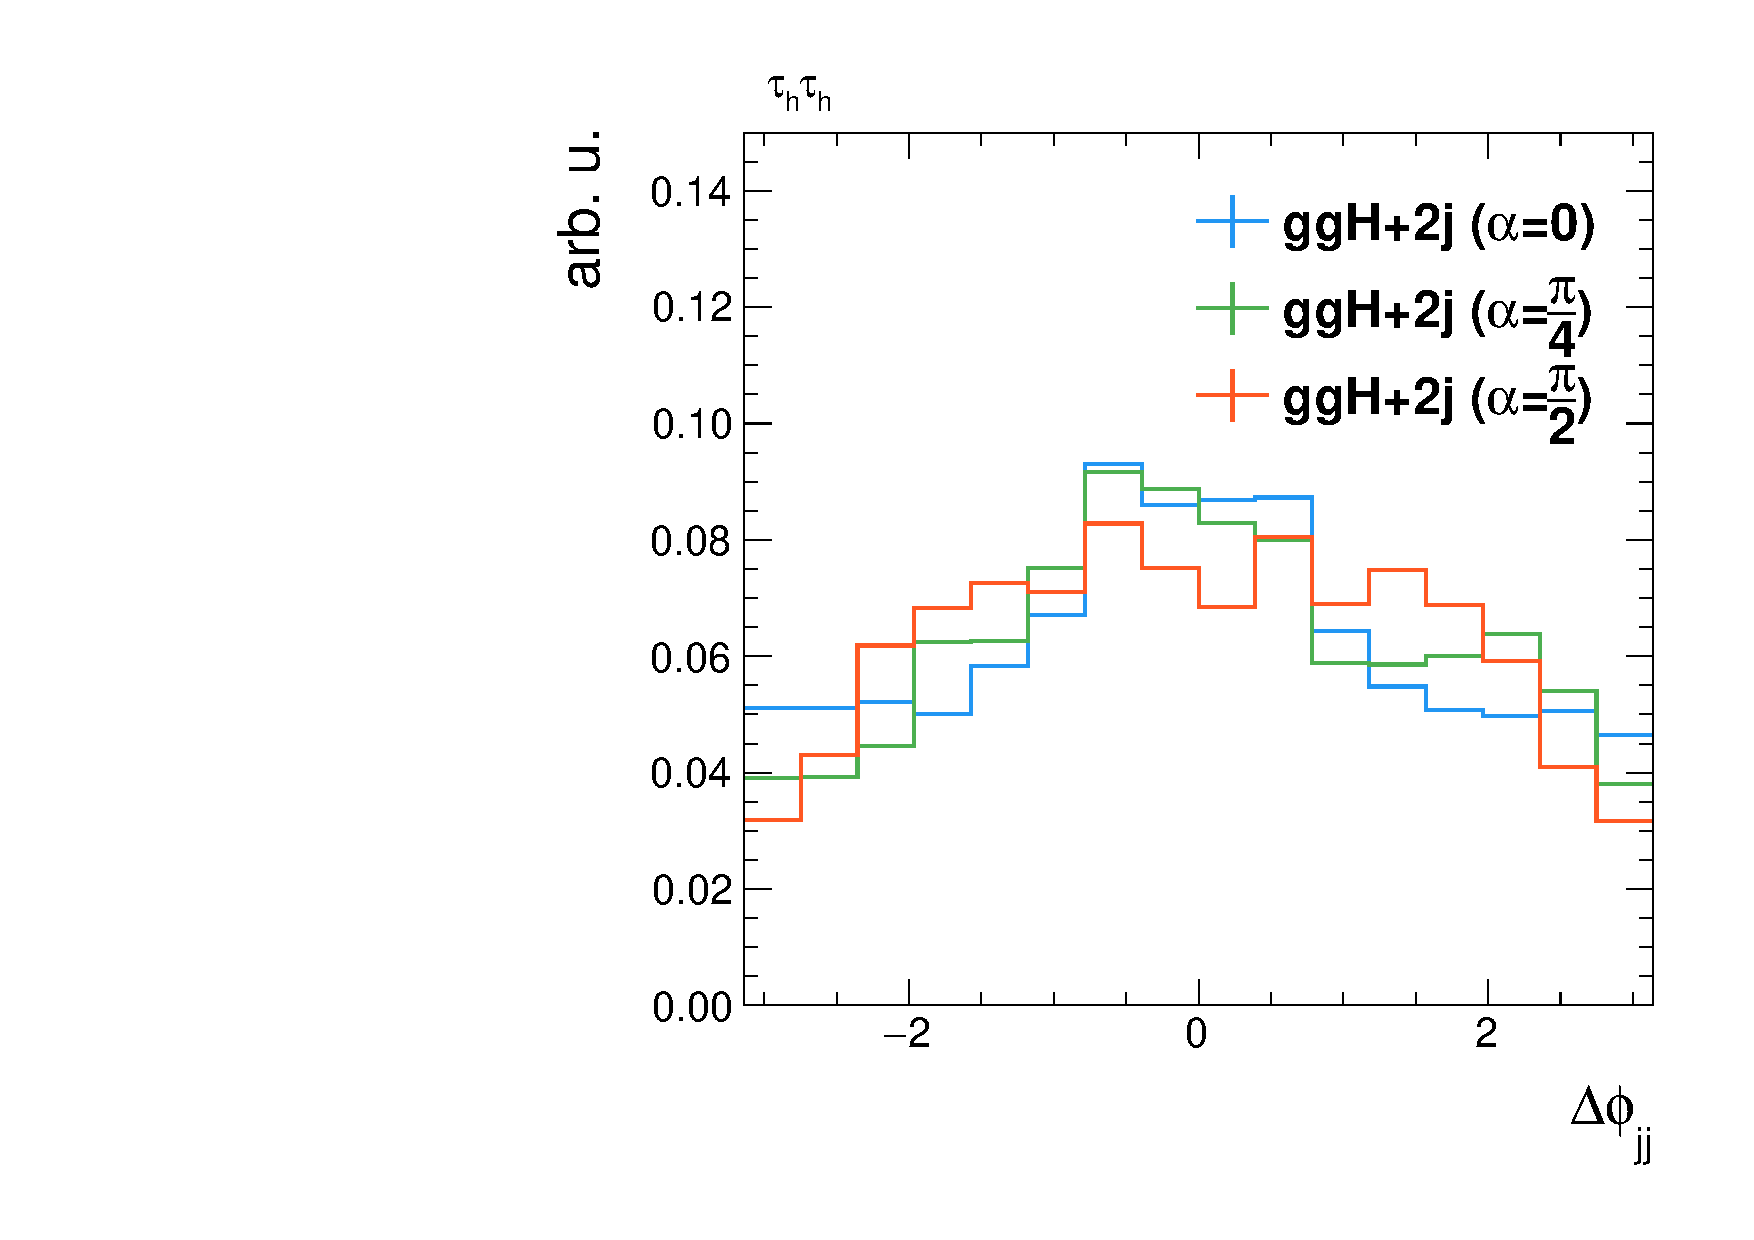
\includegraphics[width=\textwidth]{Figures/eventselection/CPHypotheses/tt/JHU_jdphi_no_cuts.pdf} %
    \end{subfigure}
    \begin{subfigure}{.45\textwidth}
        \centering
        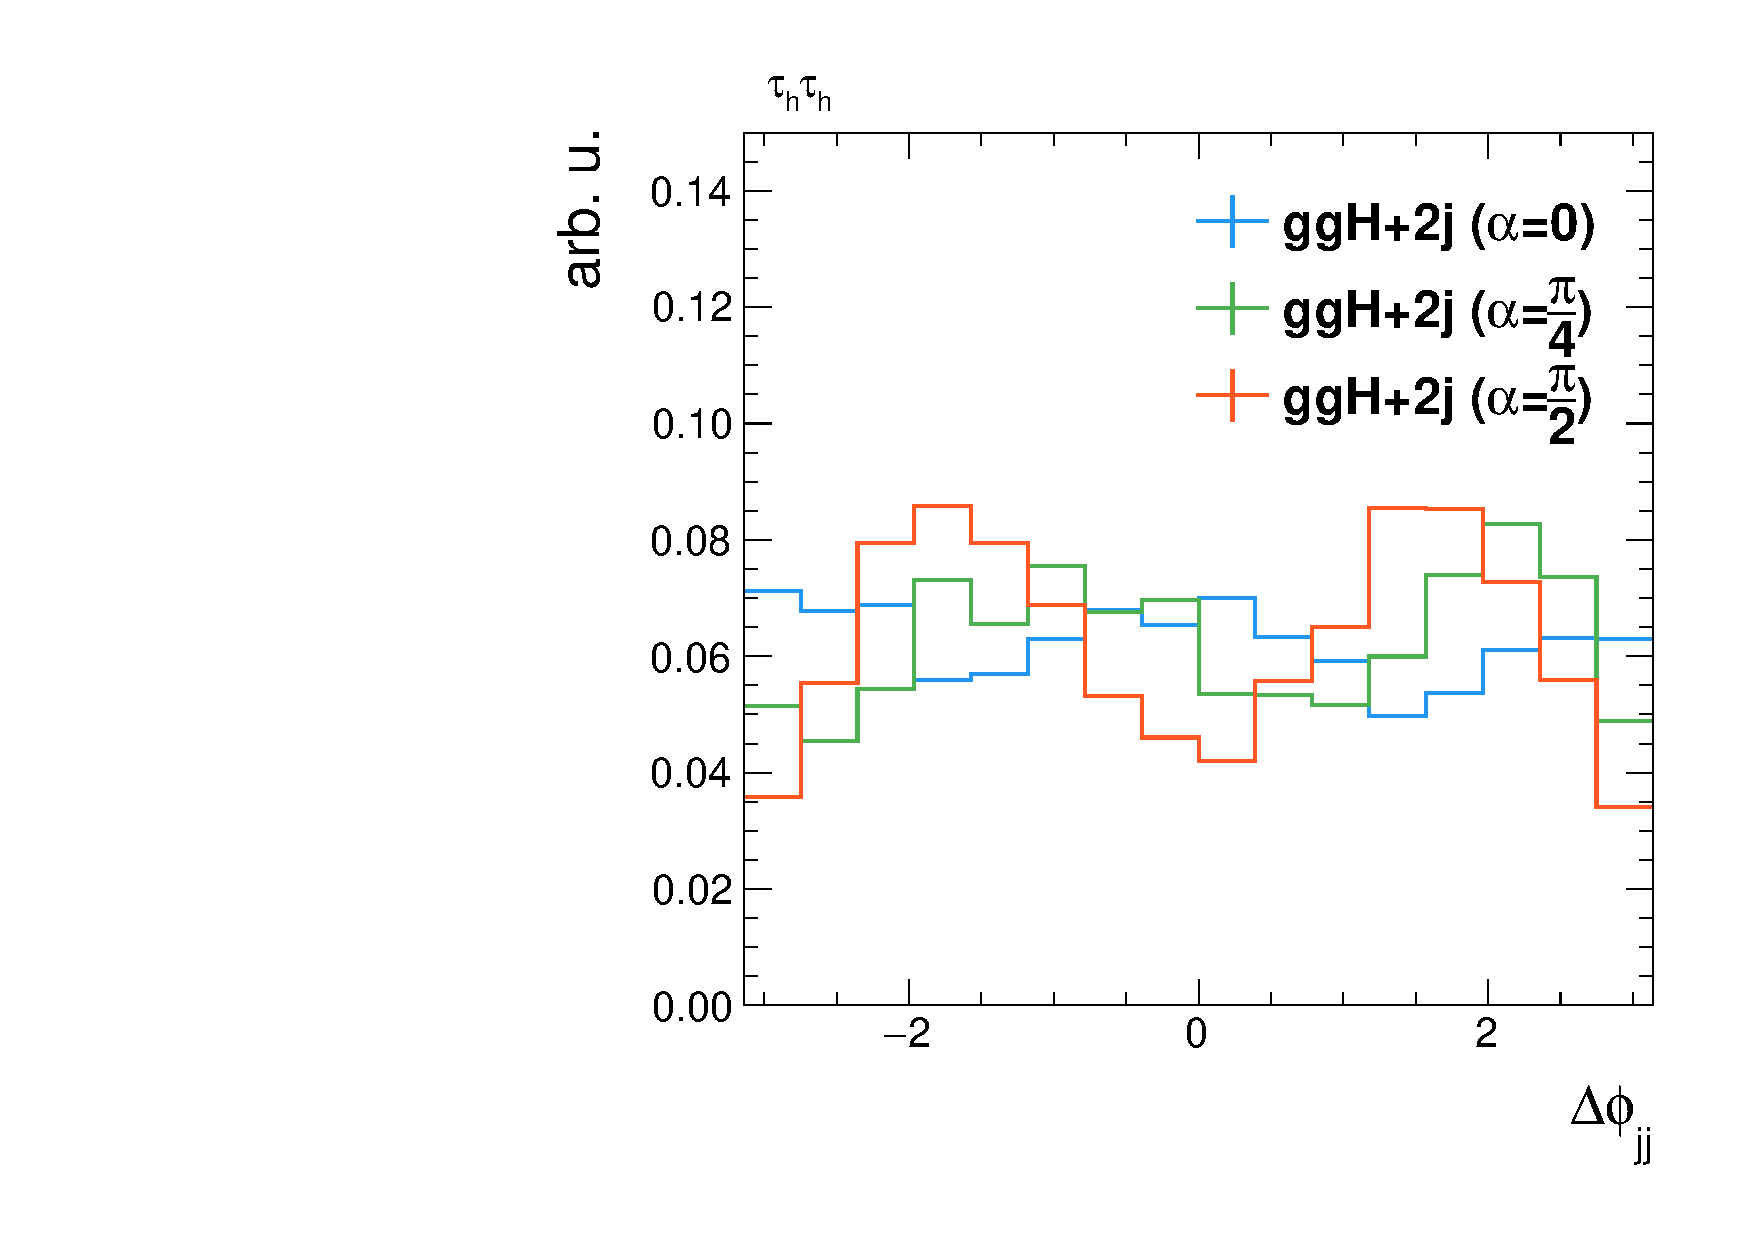
\includegraphics[width=\textwidth]{Figures/eventselection/CPHypotheses/tt/JHU_jdphi_mjj_cuts.pdf}%
    \end{subfigure}
    \caption[\jdphi{} shape comparison.]{Comparison of the normalized $\Delta \phi_\text{jj}$ distributions of three CP hypotheses in the $\tau_\text{h}\tau_\text{h}$ channel.
    Simulated events provided by the three samples generated by the JHU \@{Monte Carlo} event generator were utilized for this study.
    The left figure shows the shapes without applying any further criteria on top of the event selection requirements from \textreft{sec:baseline}.
     For the right plot events are required to have an $m_\text{jj}>\text{300\,GeV}$ yielding a better separability.}\label{ES:jdphi_shapes}%
\end{figure}%

\subsubsection{Matrix Element Likelihood Analysis (MELA)}\label{sec:MELA}
The matrix element $\mathcal{M}$ calculated by Monte Carlo generators is used to simulate the distributions
of kinematic observables. It encaptures all information about a quantum physical process and vice versa.
This fact is exploited in the Matrix Element Likelihood Approach
(MELA) that aims to project the full Higgs boson production kinematics of multiple observables into a set of only a few kinematic discriminants \cite{constrainingHiggsAtProtonColliders,spin_determination,onthespin,constrainHiggsBosonCoupingsWithMET}. This approach was already applied during the search for the Higgs boson decaying into a pair of Z bosons in Run 1 \cite{Chatrchyan2012_hzz}.
So far only one of the five angles present in \figreft{ES:event_kinematics} was examined. By means of MELA, the full information of all five angles can be exploited projected into a 1D-variable.
MELA is seeded with the Lorentz four-vector of the Higgs boson as reconstructed by the \textit{SVFit} algorithm \cite{svfit} and the jet four-vectors clustered by the \textit{anti-k\textunderscript{t}} algorithm and calculates the likelihood $\mathcal{P}$ of 
the kinematics to be compatible with the Matrix element of a given CP scenario on an event-by-event basis. These likehoods are used further to 
build ratios that are optimal variables in terms of the Neyman-Pearson-Lemma \cite{Neyman289} to distinguish between two different hypotheses.  
To be able to distinguish between scalar, pseudoscalar and CP violating couplings of Higgs bosons produced via gluon-gluon fusion two observables are needed: 
\begin{align}
    D_{0-} &= \frac{\mathcal{P}_{0+}}{\mathcal{P}_{0+} + \mathcal{P}_{0-}} \\
    D_\text{CP} &= \frac{\mathcal{P}_\text{CP violation}}{\mathcal{P}_{0+} + \mathcal{P}_{0-}} 
\end{align}
$D_{0-}$ is used to discriminate between the scalar and pseudoscalar hypotheses and is constructed from the likelihoods $\mathcal{P}_{0+}$ and $\mathcal{P}_{0-}$ to be compatible with the scalar ($J^\text{P}=0^+$) and pseudoscalar ($J^\text{P}=0^-$) matrix elements and yields a score between 0 and 1. It is expected that
$D_{0-}$ peaks at 1 for a scalar Higgs boson, where pseudoscalar events should yield lower values on average. $D_\text{CP}$ investigates a possible CP violating term using the likelihood $\mathcal{P}_\text{CP violation}$. It projects the event information into a score between $-1$ and $+1$ and is expected to possess an asymmetric shape if CP violation is present.
The distributions of both discriminators for three CP scenarios
are shown in \figreft{ES:dcpstar_shapes}. \newline{}
Here again the shapes of the three different CP hypotheses without applying any selection cuts are hard to distinguish. For this reason, the $m_\text{jj}>\text{300\,{GeV}}$ criterion is applied again  
leading to more pronounced shapes, too.
Furthermore, it is observed that all distributions peak around 0.5 implying that the event kinematics for different CP scenarios are very similar. Therefore, the likelihoods to belong to a certain CP scenario are rather equal. Nevertheless, it can be seen that the peaks for scalar and pseudoscalar couplings lie at different values (blue and orange histograms in the upper row, right plot) and that the intermediate scenario
causes an asymmetry  in the $D_\text{CP}$ distribution (green histogram right plot, bottom row). 

\subsection{Simulated samples}

This analysis is based on the data set collected during Run 2 at the LHC in 2016 corresponding to an integrated luminosity of $\text{35.9\,fb}^\text{-1}$.
Simulated samples for all backgrounds and SM Higgs bosons decaying into a pair of tau leptons were taken from the analysis for the search for $\mathsf{H\rightarrow\tau\tau}$ events in Ref. \cite{Sirunyan:2017khh}.
The signal samples were generated with the POWHEG generator and contain simulated Higgs bosons created by all production processes. This means, there are only few events with two initial-state jets provided, which make 
these POWHEG samples not extraordinary suited for the usage in this analysis, because two jets are needed to calculate the CP sensitive observables.
For this reason, three inclusive dijet samples for Higgs bosons produced via gluon-gluon fusion and decaying into tau leptons
with CP mixing angles $\alpha=0$, $\alpha=\frac{\pi}{4}$, and $\alpha=\frac{\pi}{2}$ were generated with the JHU generator \cite{constrainingHiggsAtProtonColliders,spin_determination,onthespin,constrainHiggsBosonCoupingsWithMET}.
PYTHIA 8 \cite{pythia} is used for modeling the decay of the Higgs boson into tau leptons, parton-showering, and hadronization. JHU uses only
matrix elements that were calculated at leading order (LO). By comparing the kinematic distributions of the scalar samples with a sample generated by the 
POWHEG event generator at next-to-leading order (NLO), it was found that the emission of two jets is well-described \cite{CMS-AN-17-034}.
The samples are listed in \tabreft{ES:jhu_samples_xsecs} together with the SM cross sections of the processes.
JHU assumes equal cross sections for the scalar and pseudoscalar scenarios. In the case of the intermediate scenario twice the cross section is yielded which can be inferred from equation \eqref{SA:total_yield} if the normalization are equal to one
as realized by the JHU generator. 
Command to produce the shapes for DCPStar 
% higgsplot.py -i /nfs/dust/cms/user/dwolfsch/htautau/artus/2018-08-07_18-44_Run2CPStudies_Nominal_Summer16_plusHToTauTauM110-140/merged/GluGluH2JetsToTauTauM125CPmixingsmJHU_RunIISummer16MiniAODv2_PUMoriond17_13TeV_MINIAOD_JHUgen/GluGluH2JetsToTauTauM125CPmixingsmJHU_RunIISummer16MiniAODv2_PUMoriond17_13TeV_MINIAOD_JHUgen.root /nfs/dust/cms/user/dwolfsch/htautau/artus/2018-08-07_18-44_Run2CPStudies_Nominal_Summer16_plusHToTauTauM110-140/merged/GluGluH2JetsToTauTauM125CPmixingmaxmixJHU_RunIISummer16MiniAODv2_PUMoriond17_13TeV_MINIAOD_JHUgen/GluGluH2JetsToTauTauM125CPmixingmaxmixJHU_RunIISummer16MiniAODv2_PUMoriond17_13TeV_MINIAOD_JHUgen.root  /nfs/dust/cms/user/dwolfsch/htautau/artus/2018-08-07_18-44_Run2CPStudies_Nominal_Summer16_plusHToTauTauM110-140/merged/GluGluH2JetsToTauTauM125CPmixingpseudoscalarJHU_RunIISummer16MiniAODv2_PUMoriond17_13TeV_MINIAOD_JHUgen/GluGluH2JetsToTauTauM125CPmixingpseudoscalarJHU_RunIISummer16MiniAODv2_PUMoriond17_13TeV_MINIAOD_JHUgen.root -f tt_nominal/ntuple -x melaDiscriminatorDCPGGH --x-label "D_{CP}" --x-bins "3,-1,1" --labels "ggH+2j(#alpha=0)" "ggH+2j(#alpha=#frac{#pi}{4})" "ggH+2j(#alpha=#frac{#pi}{2})"  --colors material_blue2  material_green material_orange  --analysis-modules NormalizeToUnity --title "#tau_{h}#tau_{h}" -w "(njets>1)" --y-label "arb. u." --filename "JHU_DCP_no_cuts" -m LINE --legend-markers LINE --legend --y-lims 0 1.5 --www CPHypotheses --live --line-width 2  --formats png pdf
% higgsplot.py -i /nfs/dust/cms/user/dwolfsch/htautau/artus/2018-08-07_18-44_Run2CPStudies_Nominal_Summer16_plusHToTauTauM110-140/merged/GluGluH2JetsToTauTauM125CPmixingsmJHU_RunIISummer16MiniAODv2_PUMoriond17_13TeV_MINIAOD_JHUgen/GluGluH2JetsToTauTauM125CPmixingsmJHU_RunIISummer16MiniAODv2_PUMoriond17_13TeV_MINIAOD_JHUgen.root /nfs/dust/cms/user/dwolfsch/htautau/artus/2018-08-07_18-44_Run2CPStudies_Nominal_Summer16_plusHToTauTauM110-140/merged/GluGluH2JetsToTauTauM125CPmixingmaxmixJHU_RunIISummer16MiniAODv2_PUMoriond17_13TeV_MINIAOD_JHUgen/GluGluH2JetsToTauTauM125CPmixingmaxmixJHU_RunIISummer16MiniAODv2_PUMoriond17_13TeV_MINIAOD_JHUgen.root  /nfs/dust/cms/user/dwolfsch/htautau/artus/2018-08-07_18-44_Run2CPStudies_Nominal_Summer16_plusHToTauTauM110-140/merged/GluGluH2JetsToTauTauM125CPmixingpseudoscalarJHU_RunIISummer16MiniAODv2_PUMoriond17_13TeV_MINIAOD_JHUgen/GluGluH2JetsToTauTauM125CPmixingpseudoscalarJHU_RunIISummer16MiniAODv2_PUMoriond17_13TeV_MINIAOD_JHUgen.root -f tt_nominal/ntuple -x melaDiscriminatorD0MinusGGH --x-label "D_{0-}" --x-bins "4,0,1" --labels "ggH+2j(#alpha=0)" "ggH+2j(#alpha=#frac{#pi}{4})" "ggH+2j(#alpha=#frac{#pi}{2})"  --colors material_blue2  material_green material_orange  --analysis-modules NormalizeToUnity --title "#tau_{h}#tau_{h}" -w "(njets>1)" --y-label "arb. u." --filename "JHU_D0Minus_no_cuts" -m LINE --legend-markers LINE  --legend --y-lims 0 1.0 --www CPHypotheses --live --line-width 2  --formats png pdf
% higgsplot.py -i /nfs/dust/cms/user/dwolfsch/htautau/artus/2018-08-07_18-44_Run2CPStudies_Nominal_Summer16_plusHToTauTauM110-140/merged/GluGluH2JetsToTauTauM125CPmixingsmJHU_RunIISummer16MiniAODv2_PUMoriond17_13TeV_MINIAOD_JHUgen/GluGluH2JetsToTauTauM125CPmixingsmJHU_RunIISummer16MiniAODv2_PUMoriond17_13TeV_MINIAOD_JHUgen.root /nfs/dust/cms/user/dwolfsch/htautau/artus/2018-08-07_18-44_Run2CPStudies_Nominal_Summer16_plusHToTauTauM110-140/merged/GluGluH2JetsToTauTauM125CPmixingmaxmixJHU_RunIISummer16MiniAODv2_PUMoriond17_13TeV_MINIAOD_JHUgen/GluGluH2JetsToTauTauM125CPmixingmaxmixJHU_RunIISummer16MiniAODv2_PUMoriond17_13TeV_MINIAOD_JHUgen.root  /nfs/dust/cms/user/dwolfsch/htautau/artus/2018-08-07_18-44_Run2CPStudies_Nominal_Summer16_plusHToTauTauM110-140/merged/GluGluH2JetsToTauTauM125CPmixingpseudoscalarJHU_RunIISummer16MiniAODv2_PUMoriond17_13TeV_MINIAOD_JHUgen/GluGluH2JetsToTauTauM125CPmixingpseudoscalarJHU_RunIISummer16MiniAODv2_PUMoriond17_13TeV_MINIAOD_JHUgen.root -f tt_nominal/ntuple -x melaDiscriminatorDCPGGH --x-label "D_{CP}" --x-bins "3,-1,1" --labels "ggH+2j(#alpha=0)" "ggH+2j(#alpha=#frac{#pi}{4})" "ggH+2j(#alpha=#frac{#pi}{2})"  --colors material_blue2  material_green material_orange  --analysis-modules NormalizeToUnity --title "#tau_{h}#tau_{h}" -w "(njets>1)*(mjj>300)" --y-label "arb. u." --filename "JHU_DCP_mjj_cuts" -m LINE --legend-markers LINE  --legend --y-lims 0 1.5 --www CPHypotheses --live --line-width 3 --formats png pdf
% higgsplot.py -i /nfs/dust/cms/user/dwolfsch/htautau/artus/2018-08-07_18-44_Run2CPStudies_Nominal_Summer16_plusHToTauTauM110-140/merged/GluGluH2JetsToTauTauM125CPmixingsmJHU_RunIISummer16MiniAODv2_PUMoriond17_13TeV_MINIAOD_JHUgen/GluGluH2JetsToTauTauM125CPmixingsmJHU_RunIISummer16MiniAODv2_PUMoriond17_13TeV_MINIAOD_JHUgen.root /nfs/dust/cms/user/dwolfsch/htautau/artus/2018-08-07_18-44_Run2CPStudies_Nominal_Summer16_plusHToTauTauM110-140/merged/GluGluH2JetsToTauTauM125CPmixingmaxmixJHU_RunIISummer16MiniAODv2_PUMoriond17_13TeV_MINIAOD_JHUgen/GluGluH2JetsToTauTauM125CPmixingmaxmixJHU_RunIISummer16MiniAODv2_PUMoriond17_13TeV_MINIAOD_JHUgen.root  /nfs/dust/cms/user/dwolfsch/htautau/artus/2018-08-07_18-44_Run2CPStudies_Nominal_Summer16_plusHToTauTauM110-140/merged/GluGluH2JetsToTauTauM125CPmixingpseudoscalarJHU_RunIISummer16MiniAODv2_PUMoriond17_13TeV_MINIAOD_JHUgen/GluGluH2JetsToTauTauM125CPmixingpseudoscalarJHU_RunIISummer16MiniAODv2_PUMoriond17_13TeV_MINIAOD_JHUgen.root -f tt_nominal/ntuple -x melaDiscriminatorD0MinusGGH --x-label "D_{0-}" --x-bins "4,0,1" --labels "ggH+2j(#alpha=0)" "ggH+2j(#alpha=#frac{#pi}{4})" "ggH+2j(#alpha=#frac{#pi}{2})"  --colors material_blue2  material_green material_orange  --analysis-modules NormalizeToUnity --title "#tau_{h}#tau_{h}" -w "(njets>1)*(mjj>300)" --y-label "arb. u." --filename "JHU_D0Minus_mjj_cuts" -m LINE --legend-markers LINE  --legend --y-lims 0 1.0 --www CPHypotheses --live --line-width 3 --formats png pdf

\begin{figure}[h!]
   \centering
   \begin{subfigure}{.49\textwidth}
       \centering
       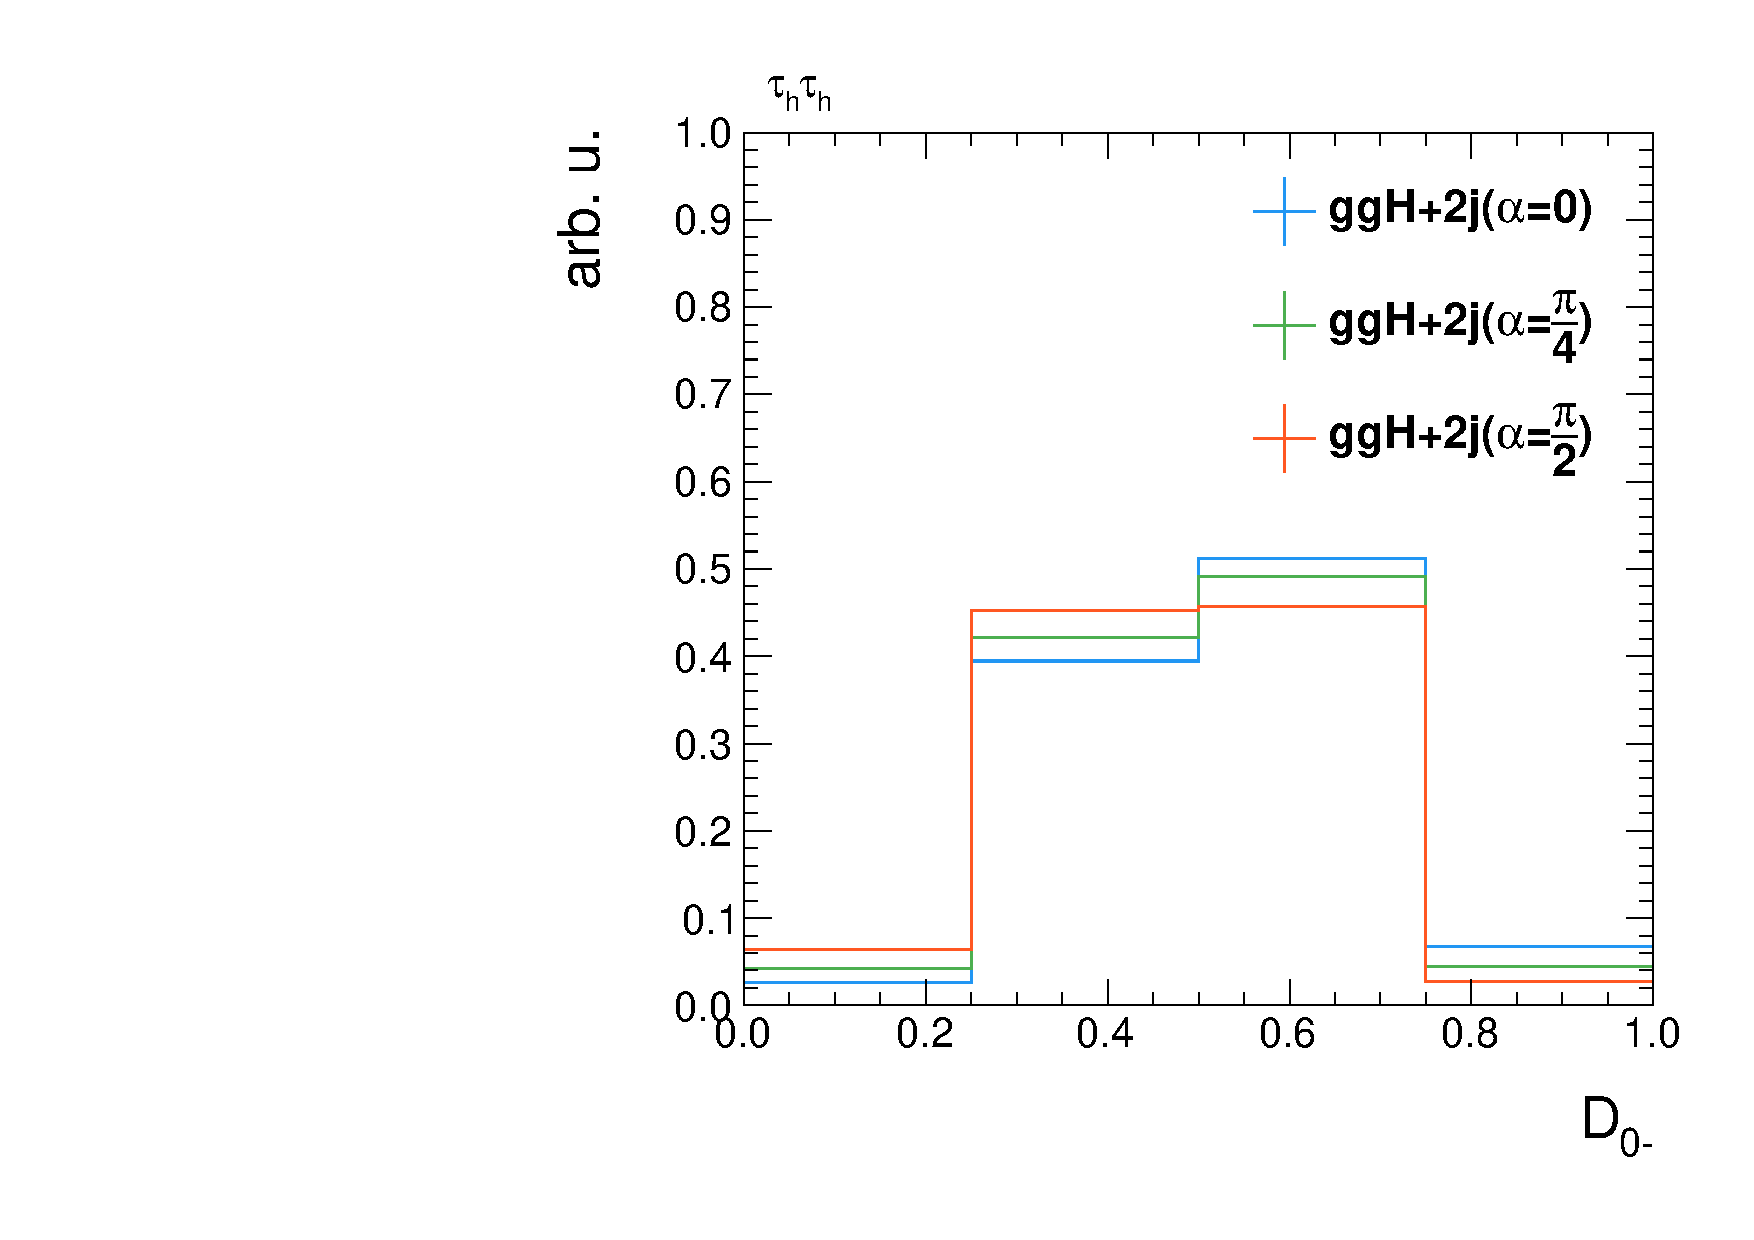
\includegraphics[width=\textwidth]{Figures/eventselection/CPHypotheses/JHU_D0Minus_no_cuts.pdf}%
   \end{subfigure}
   \begin{subfigure}{.49\textwidth}
       \centering
       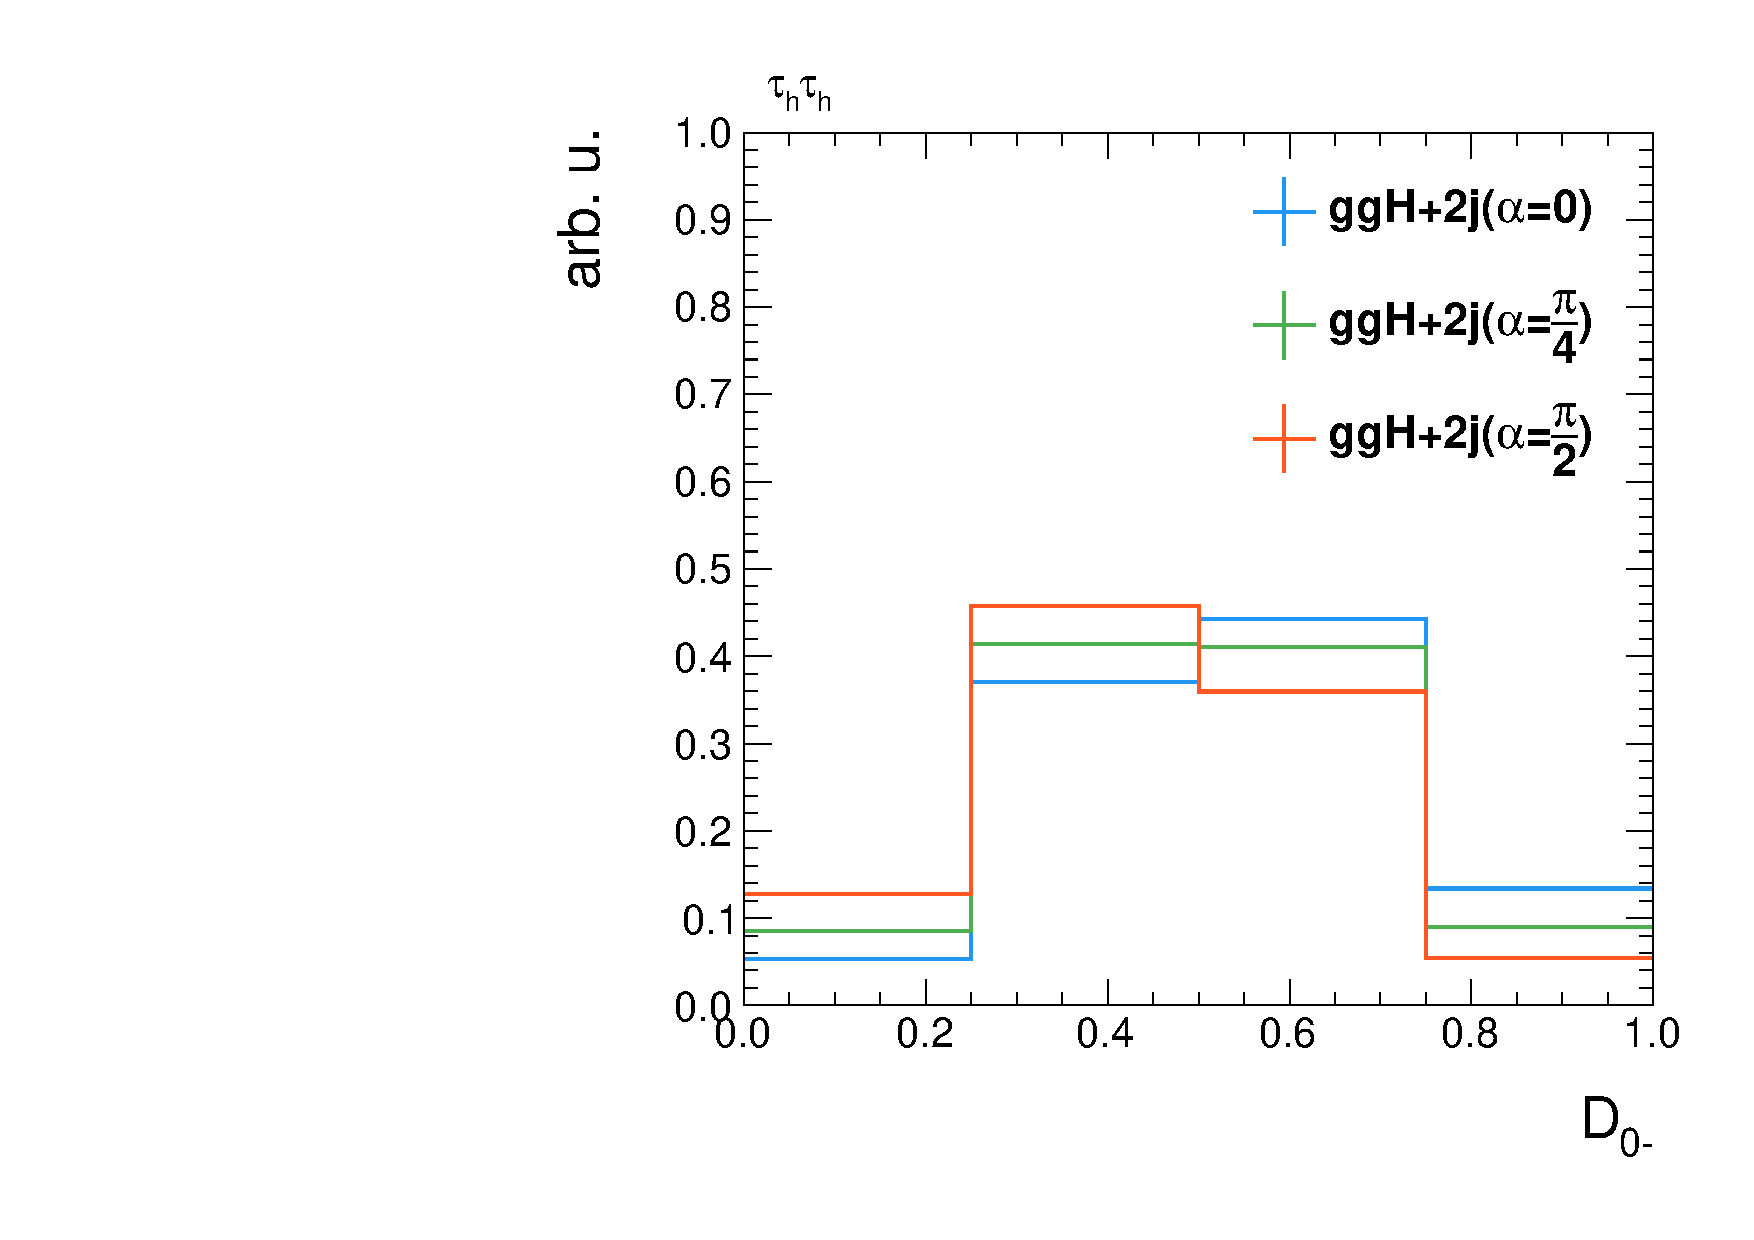
\includegraphics[width=\textwidth]{Figures/eventselection/CPHypotheses/JHU_D0Minus_mjj_cuts.pdf} \\%
   \end{subfigure}
   \begin{subfigure}{.49\textwidth}
       \centering
       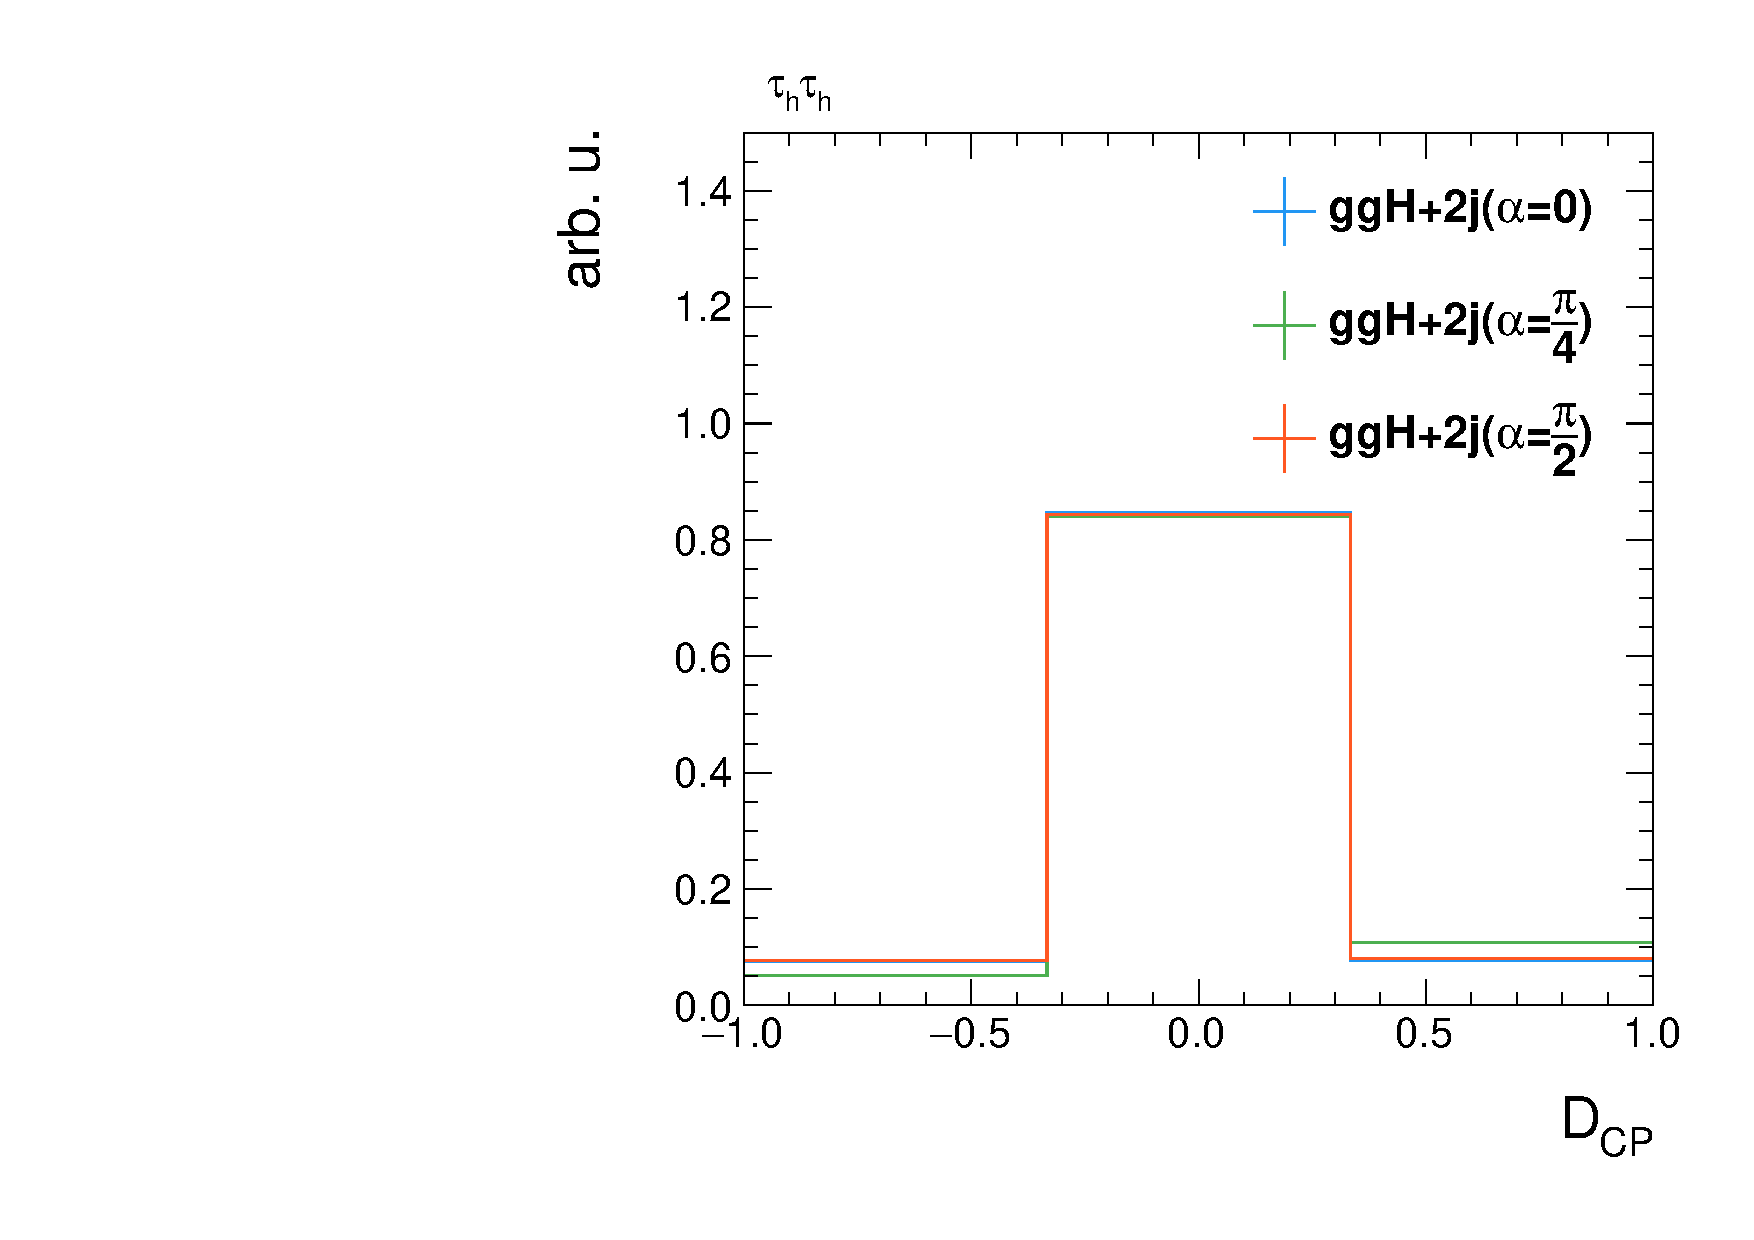
\includegraphics[width=\textwidth]{Figures/eventselection/CPHypotheses/JHU_DCP_no_cuts.pdf}%
   \end{subfigure}
   \begin{subfigure}{.49\textwidth}
       \centering
       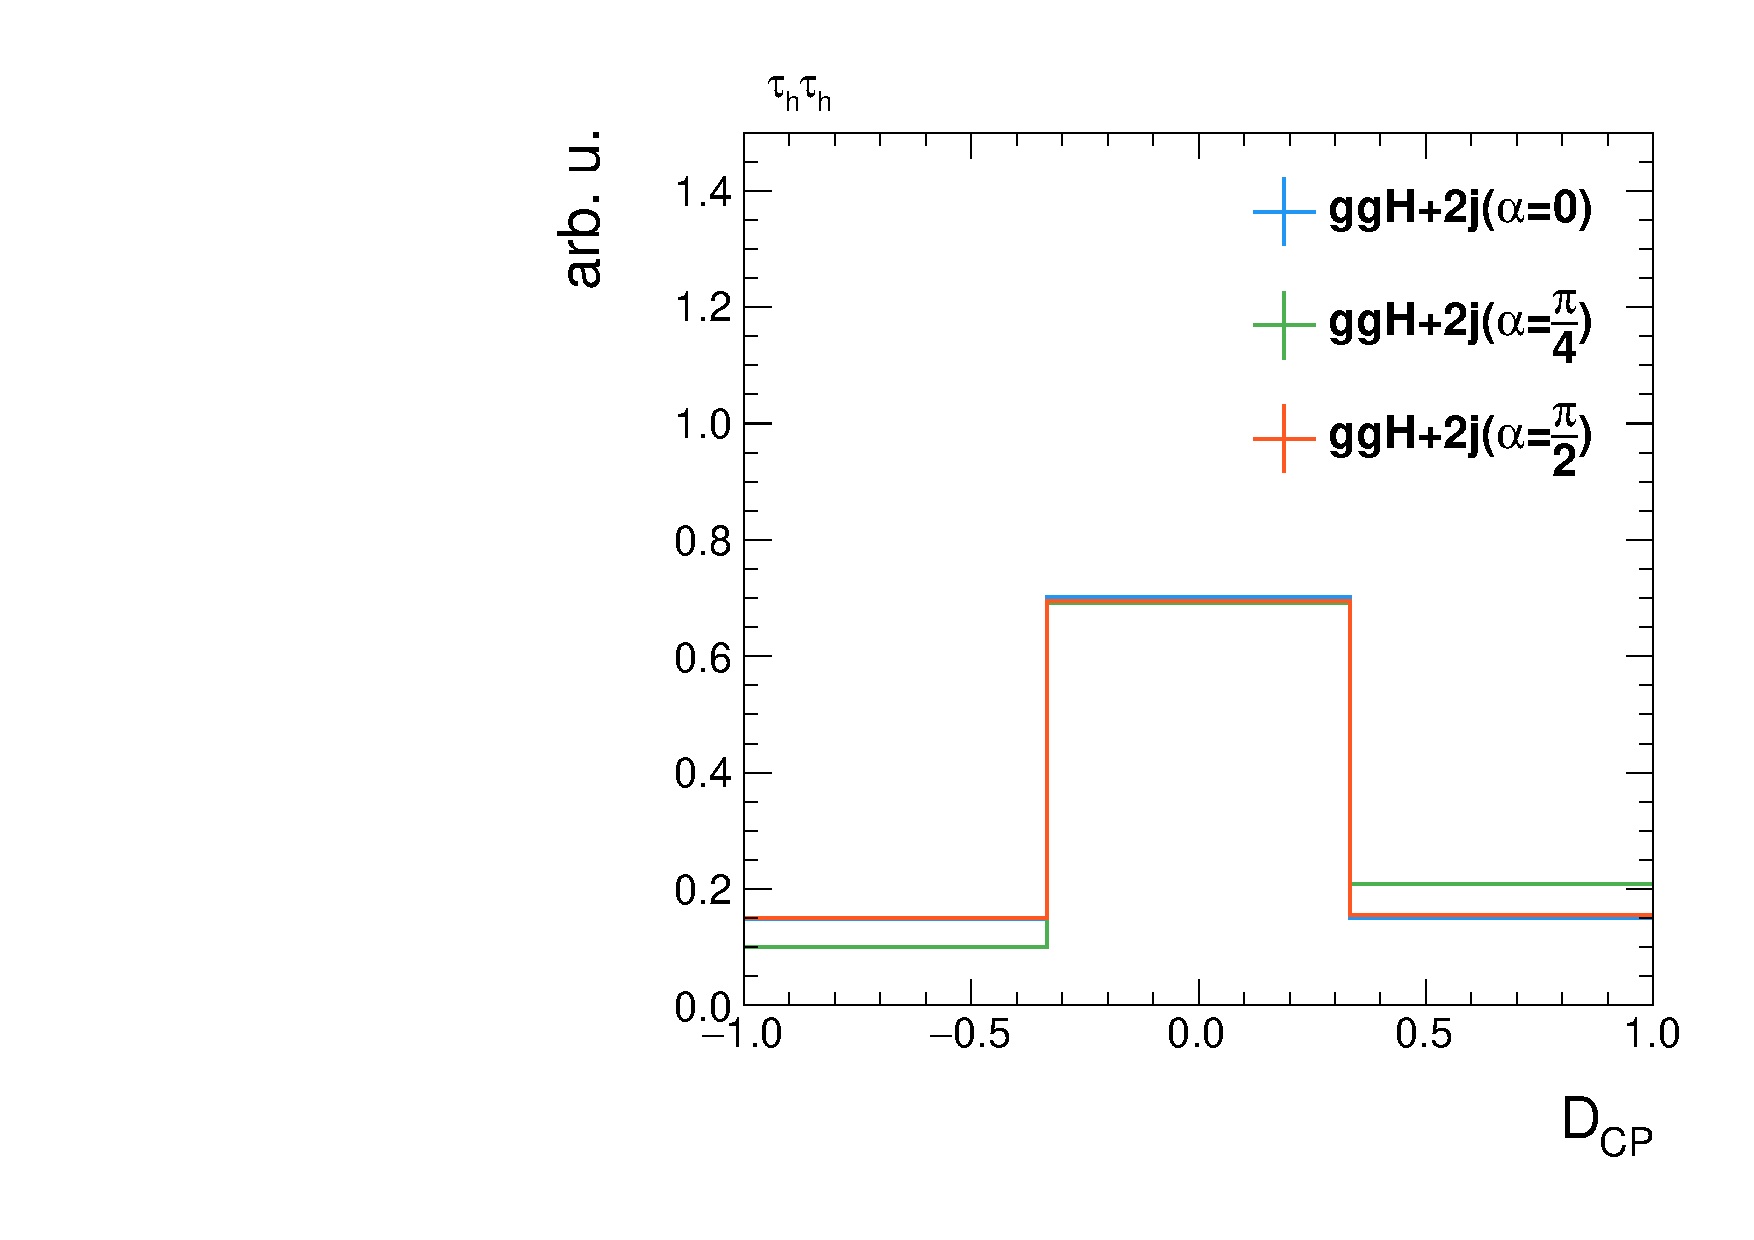
\includegraphics[width=\textwidth]{Figures/eventselection/CPHypotheses/JHU_DCP_mjj_cuts.pdf} \\%
   \end{subfigure}    
   \caption[$D_{0-}$ and $D_\text{CP}$ shape comparison.]{Comparison of the normalized $D_{0-}$ (upper row) and $D_\text{CP}$ (bottom row) distributions for three CP scenarios in the $\tau_\text{h}\tau_\text{h}$ channel. Simulated events generated by the JHU Monte Carlo event generator where utilized to predict the shapes. The left plots shows the distribution without any further criteria on top of those defined 
   in \textreft{sec:baseline} are used. For the right plot events are required to satisfy $m_\text{jj}>\text{300\,{GeV}}$ yielding a better separation between the different hypotheses.
   With the $m_\text{jj}$ criterion the peak of the different CP scenarios in $D_{0-}$ (right plot, upper row) lies in neighboring bins around $\text{0.5}$. This means the different CP scenarios have very similar shapes. Three bins are used in $D_\text{CP}$ to put emphasis on events that were well reconstructed and lie therefore in the tails of the distribution.  
   The CP violating scenario shows here an asymmetry, whereas the pure states cannot be distinguished (right plot, bottom row).}\label{ES:dcpstar_shapes}%
\end{figure}%
\newpage{}
% https://twiki.cern.ch/twiki/bin/viewauth/CMS/Run2MCProductionforHiggsProperties
\begin{table}[h]
    \centering
    \caption[Simulated JHU signal samples.]{Gluon-gluon fusion in association with two jets and VBF samples generated by the JHU generator used in this analysis. Events
    are generated with an increased cross section and later normalized to SM cross section \cite{Patrignani:2016xqp}.}\label{ES:jhu_samples_xsecs} 
    \begin{tabular}{llll}
        \toprule
        Name                                              & Events &  $\sigma_{SM}$/pb \\
        \midrule
        { GluGluH2JetsToTauTau\_M125\_13TeV\_CPmixing\_sm\_JHU          }  & $\text{10}^\text{6}$ & 0.399 \\
        { GluGluH2JetsToTauTau\_M125\_13TeV\_CPmixing\_maxmix\_JHU      }  & $\text{10}^\text{6}$ & 0.789 \\
        { GluGluH2JetsToTauTau\_M125\_13TeV\_CPmixing\_pseudoscalar\_JHU}  & $\text{10}^\text{6}$ & 0.386 \\
        \midrule
        { VBFHiggs0PM\_M-125\_13TeV-JHUGenV6           }                   & $\text{10}^\text{6}$ & 2.671 \\
        { VBFHiggs0Mf05ph0\_M-125 13TeV-JHUGenV6       }                   & $\text{10}^\text{6}$ & 0.474 \\
        { VBFHiggs0MM\_M-125\_13TeV-JHUGenV6           }                   & $\text{10}^\text{6}$ & 0.237 \\ \bottomrule
    \end{tabular}%
\end{table}%

\subsection{Categorization}\label{sec:categorization}
Previously, it has been found that a simple requirement on $m_\text{jj}$ leads to better distinguishability between the three signal samples. 
This motivates that there are regions of phase space that provide a better separation between these samples than the overall separation in an inclusive event selection. Moreover, the selection of 
events is not pure in Higgs boson events. The baseline selection comes with a large contamination of background events which have signatures that mimick the signal in the detector. In this section, additional quality requirements are introduced to separate signal from background.
Another goal here is to increase the fraction of selected Higgs bosons generated by ggF compared to VBF produced Higgs bosons in the signal categories to be sensitive to fermionic couplings.
In this analysis events, that pass the baseline selection, are split into four categories to maximize the sensitivity to measure the CP properties in the fermionic couplings. 
For this purpose, the categories defined for \cite{Sirunyan:2017khh} are adapted and optimized.

\subsubsection{0-jet and boosted categories}

\begin{table}[!]
    \centering
    \caption[Selection cuts \textit{0-jet} and \textit{boosted} categories.]{Selection cuts and observables of the \textit{0-jet} and \textit{boosted} categories used within this analysis.}\label{ES:categorization_0jet1jet}
    \begin{tabular}{lll}
        \toprule
        Channel         & 0-jet         & boosted    \\ \midrule
        \multicolumn{3}{c}{Selection cuts}                                                       \\ \hline
        $e\mu$,$e\tau_\text{h}$,$\mu\tau_\text{h}$           & No jet \& No b-jet  &  \multirow{2}{*}{Not in 0-jet \& not in dijet}        \\                
        $\tau_\text{h}\tau_\text{h}$  &  No jet                                 &          \\\midrule     
        \multicolumn{3}{c}{Observables}                                         \\ \midrule
        All          &  $m_{\tau\tau}$                            &  $m_{\tau\tau}\times p_\text{\,T}^{\tau\tau}$  \\    \bottomrule                                                                         
    \end{tabular}
\end{table}

Events with no jets fall into the \textit{0-jet} category. All events that have either one jet or a dijet system without an invariant dijet mass greater than $m_\text{jj}=\text{300\,{GeV}}$ fall into the \textit{boosted} category. 
Since signal events are required to have at least two jets, these two categories serve as background containers, that help to control the contamination of backgrounds and nuisance parameters
in the signal categories during the final fit. The requirements for these two categories are summarzied in \tabreft{ES:categorization_0jet1jet}.
Compared to Ref. \cite{Sirunyan:2017khh}, a b-tag veto is added to the $e\mu$, $e\tau_\text{h}$ and $\mu\tau_\text{h}$ channels to further reduce the contamination from top-anti-top quark production, $t\bar{t}$. 
Moreover, events in the \textit{0-jet} category are no longer discriminated in bins of the reconstructed tau decay mode but remain to be examined using the reconstructed invariant ditau mass $m_{\tau\tau}$. This has the advantage that 
the five associated decay-mode specific systematic uncertainties listed in \tabreft{tab:redundant} become redundant. \\
$m_{\tau\tau}$ is the full invariant ditau mass as reconstructed by the \textit{SVFit} algorithm. As shown in \figreft{ES:controlplots:0jet_boosted} the \textit{SVFit} mass is 
capable of separating the Z and the Higgs boson resonances and is thus a powerful discriminant to reject Drell-Yan (DY) background events. 
For the \textit{boosted} category a two-dimensional discriminator is chosen in bins of $m_{\tau\tau}$ and the $p_\text{\,T}$ of the Higgs boson, that is constructed from the reconstructed four-momenta of the two taus and the missing transverse energy
\begin{equation}
    \vec{p}_{\text{T}}^{\tau\tau}=  \vec{p}_{\text{\,T}} \li \tau_1 \re + \vec{p}_{\text{\,T}} \li \tau_2 \re + \vec{E}_\text{T}^\text{miss}.
\end{equation}
\begin{table}[h]
    \centering
    \caption[Selection cuts \textit{0-jet} and \textit{boosted} categories.]{Selection cuts and observables of the \textit{0-jet} and \textit{boosted} categories used within this analysis.}\label{ES:categorization_0jet1jet}
    \begin{tabular}{lll}
        \toprule
        Channel         & 0-jet         & boosted    \\ \midrule
        \multicolumn{3}{c}{Selection cuts}                                                       \\ \hline
        $e\mu$,$e\tau_\text{h}$,$\mu\tau_\text{h}$           & No jet \& No b-jet  &  \multirow{2}{*}{Not in 0-jet \& not in dijet}        \\                
        $\tau_\text{h}\tau_\text{h}$  &  No jet                                 &          \\\midrule     
        \multicolumn{3}{c}{Observables}                                         \\ \midrule
        All          &  $m_{\tau\tau}$                            &  $m_{\tau\tau}\times p_\text{\,T}^{\tau\tau}$  \\  \bottomrule                                                                           
    \end{tabular}%
\end{table}%
For the ggF signal in the \textit{0-jet} and \textit{boosted} categories POWHEG samples are utilized because the JHU samples are inclusive dijet samples and therefore not usable for these categories. 
An overlap with dijet events with $m_\text{jj} < \text{300\,{GeV}}$ is prevented by using only events from the POWHEG samples in the \textit{boosted} category. 
The modeling of the backgrounds and ggF signal is estimated with the methods described in section \ref{sec:background_estimation}. They are shown in \figreft{ES:controlplots:0jet_boosted} for the  $\tau_\text{h}\tau_\text{h}$ channel.

\begin{table}[!]
    \centering
    \caption[Removed tau decay mode systematic uncertainties.]{Decay-mode specific systematic uncertainties that are removed from this analysis because the decay mode of the tau leptons is no longer
    used as an observable in the \textit{0-jet} category.}\label{tab:redundant} 
    \begin{tabular}{l}
        \toprule
        Name                        \\
        \midrule
        CMS\_tauDMReco\_1prong\_13TeV             \\
        CMS\_tauDMReco\_1prong1pizero\_13TeV        \\
        CMS\_tauDMReco\_3prong\_13TeV \\ \bottomrule
    \end{tabular}%
\end{table}%

%Commands for plotting the m_sv and H_pt distributions in 0jet and 1jet
% makePlots_controlPlots.py -i /nfs/dust/cms/user/dwolfsch/htautau/artus/2018-08-07_18-44_Run2CPStudies_Nominal_Summer16_plusHToTauTauM110-140/merged/ -s ztt zll ttj vv wj qcd qqh ggh -x m_sv -c tt --categories ZeroJetCP -a " --live --formats pdf  --x-bins \" 0 50 60 70 80 90 100 110 120 130 140 150 160 170 180 190 200 210 220 230 240 250 260 270 280 290 300 \" --y-subplot-label "Fraction"   " --www EventSelection --cpggh --background-method simeqn --ratio-subplot
% makePlots_controlPlots.py -i /nfs/dust/cms/user/dwolfsch/htautau/artus/2018-08-07_18-44_Run2CPStudies_Nominal_Summer16_plusHToTauTauM110-140/merged/ -s ztt zll ttj vv wj qcd qqh ggh -x m_sv -c em et mt --categories ZeroJetCP -a " --live --formats pdf  --x-bins \" 0 50 60 70 80 90 100 110 120 130 140 150 160 170 180 190 200 220 240 260 280 300 \" --y-subplot-label "Fraction"   " --www EventSelection --cpggh --background-method simeqn --ratio-subplot 
% makePlots_controlPlots.py -i /nfs/dust/cms/user/dwolfsch/htautau/artus/2018-08-07_18-44_Run2CPStudies_Nominal_Summer16_plusHToTauTauM110-140/merged/ -s ztt zll ttj vv wj qcd qqh ggh -x m_sv -c em et mt --categories BoostedCP -a " --live --formats pdf  --x-bins \" 0 80 90 100 110 120 130 140 150 160 300 \" --y-subplot-label "Fraction" --y-label "Events/bin"   " --www EventSelection --cpggh --background-method simeqn --ratio-subplot --analysis-modules NormalizeByBinWidth
% makePlots_controlPlots.py -i /nfs/dust/cms/user/dwolfsch/htautau/artus/2018-08-07_18-44_Run2CPStudies_Nominal_Summer16_plusHToTauTauM110-140/merged/ -s ztt zll ttj vv wj qcd qqh ggh -x m_sv -c tt --categories BoostedCP -a " --live --formats pdf  --x-bins \" 0 40 60 70 80 90 100 110 120 130 150 200 250 \" --y-subplot-label "Fraction" --y-label "Events/bin"   " --www EventSelection --cpggh --background-method simeqn --ratio-subplot --analysis-modules NormalizeByBinWidth
% makePlots_controlPlots.py -i /nfs/dust/cms/user/dwolfsch/htautau/artus/2018-08-07_18-44_Run2CPStudies_Nominal_Summer16_plusHToTauTauM110-140/merged/ -s ztt zll ttj vv wj qcd qqh ggh -x H_pt -c tt --categories BoostedCP -a " --live --formats pdf --y-subplot-label "Fraction" --y-label "Events/bin"   --x-bins \" 0 100 170 300 \" " --www EventSelection --cpggh --background-method simeqn --ratio-subplot --analysis-modules NormalizeByBinWidth
% makePlots_controlPlots.py -i /nfs/dust/cms/user/dwolfsch/htautau/artus/2018-08-07_18-44_Run2CPStudies_Nominal_Summer16_plusHToTauTauM110-140/merged/ -s ztt zll ttj vv wj qcd qqh ggh -x H_pt -c em et mt --categories BoostedCP -a " --live --formats pdf --y-subplot-label "Fraction" --y-label "Events/bin"  --x-bins \" 0 100 150 200 250 300 1000 \" " --www EventSelection --cpggh --background-method simeqn --ratio-subplot --analysis-modules NormalizeByBinWidth
\begin{figure}[h!]
    \centering
    \begin{subfigure}{.32\textwidth}
        \centering
        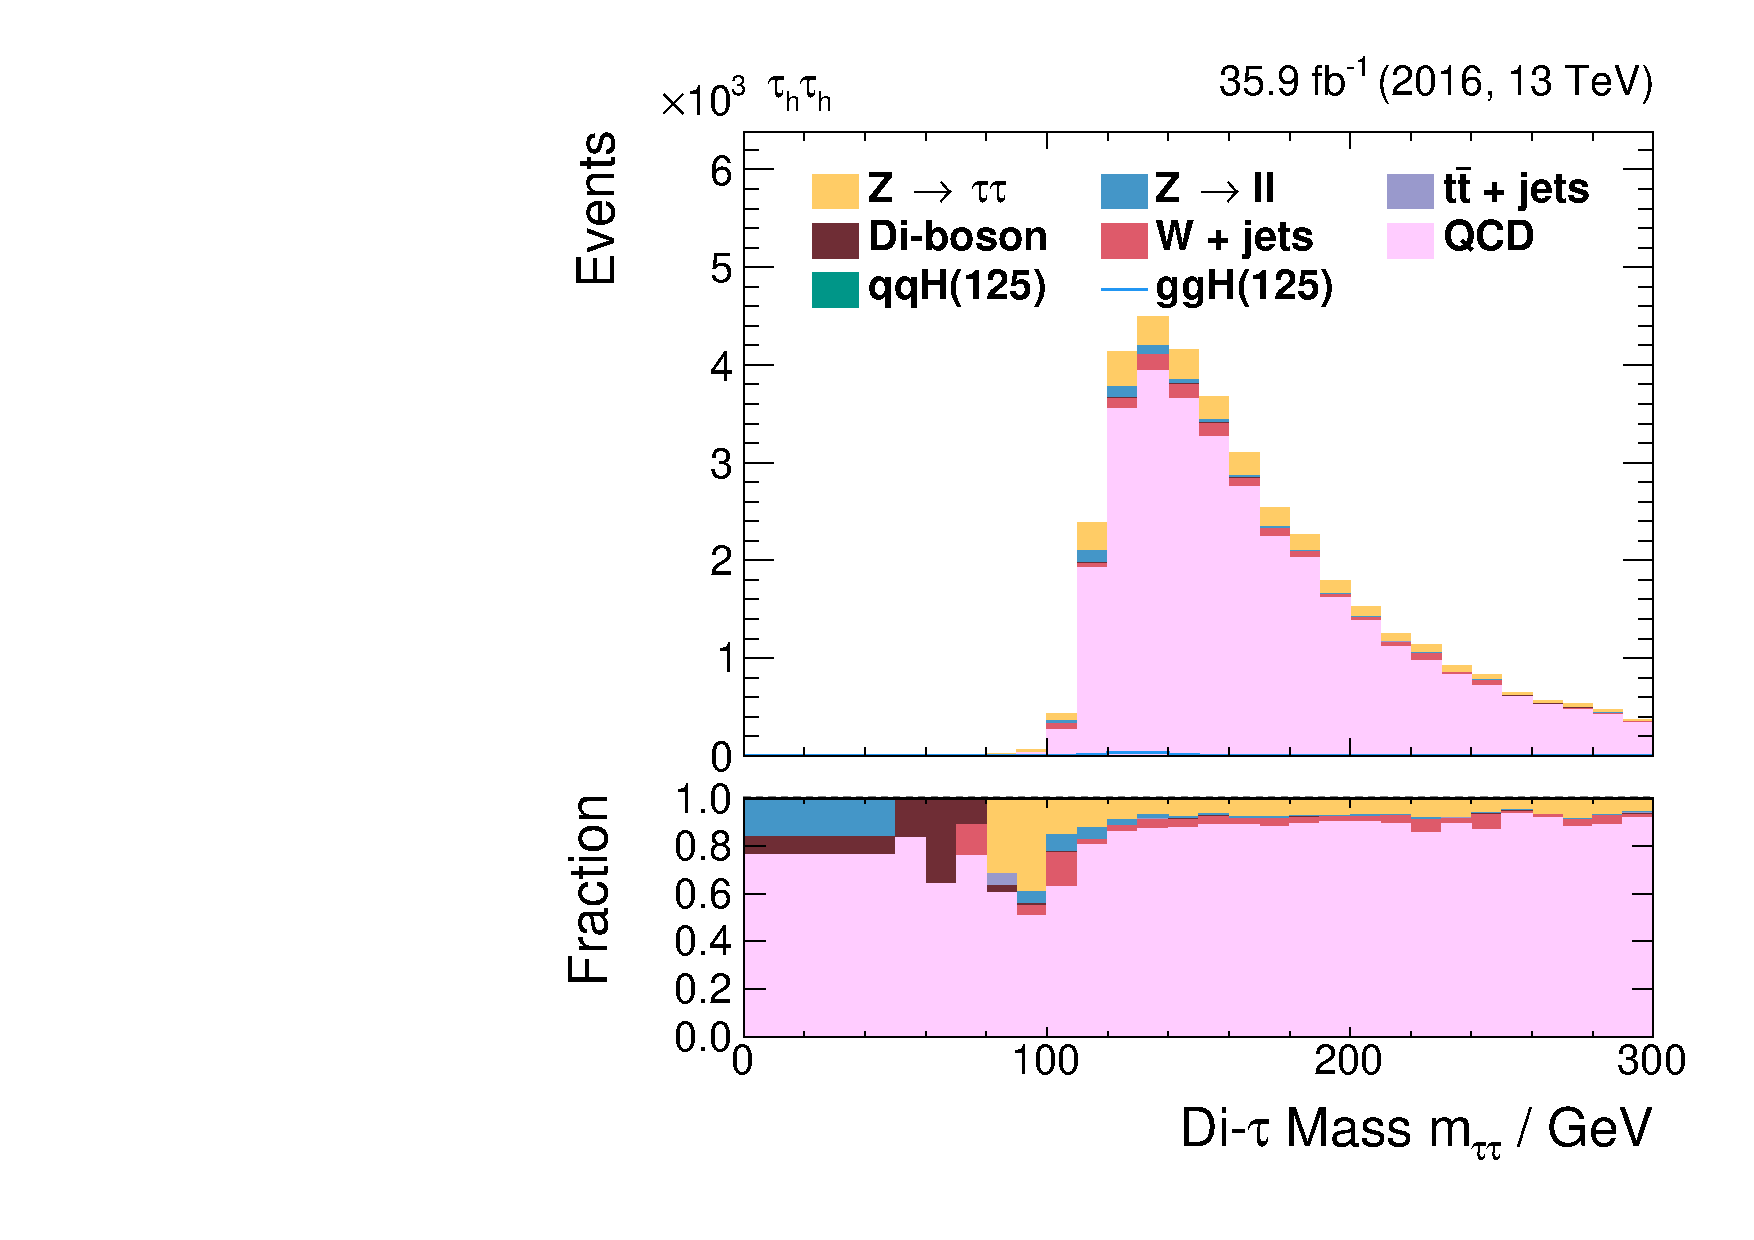
\includegraphics[width=\textwidth]{Figures/eventselection/tt/ZeroJetCP/m_sv.pdf}
    \end{subfigure}%
    \begin{subfigure}{.32\textwidth}
        \centering
        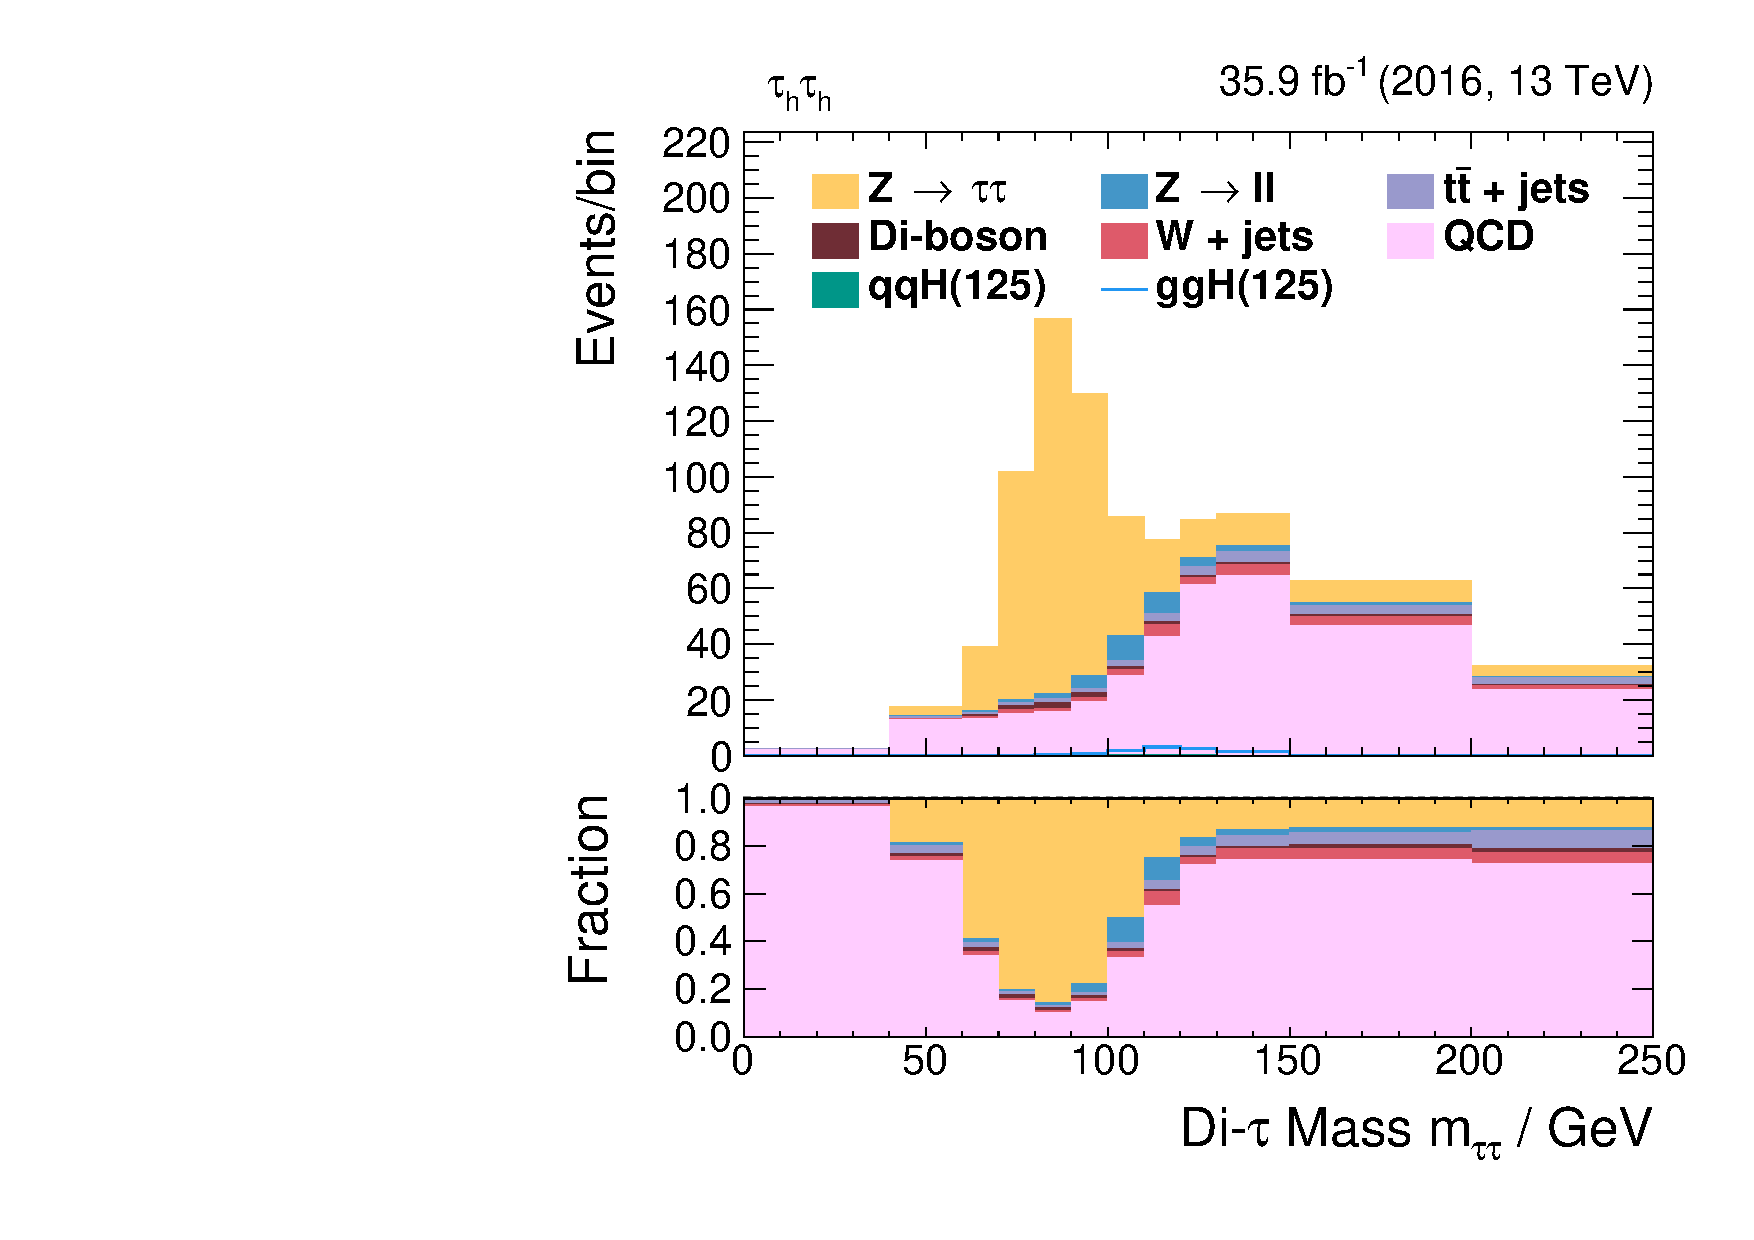
\includegraphics[width=\textwidth]{Figures/eventselection/tt/BoostedCP/m_sv.pdf}
    \end{subfigure}%
    \begin{subfigure}{.32\textwidth}
        \centering
        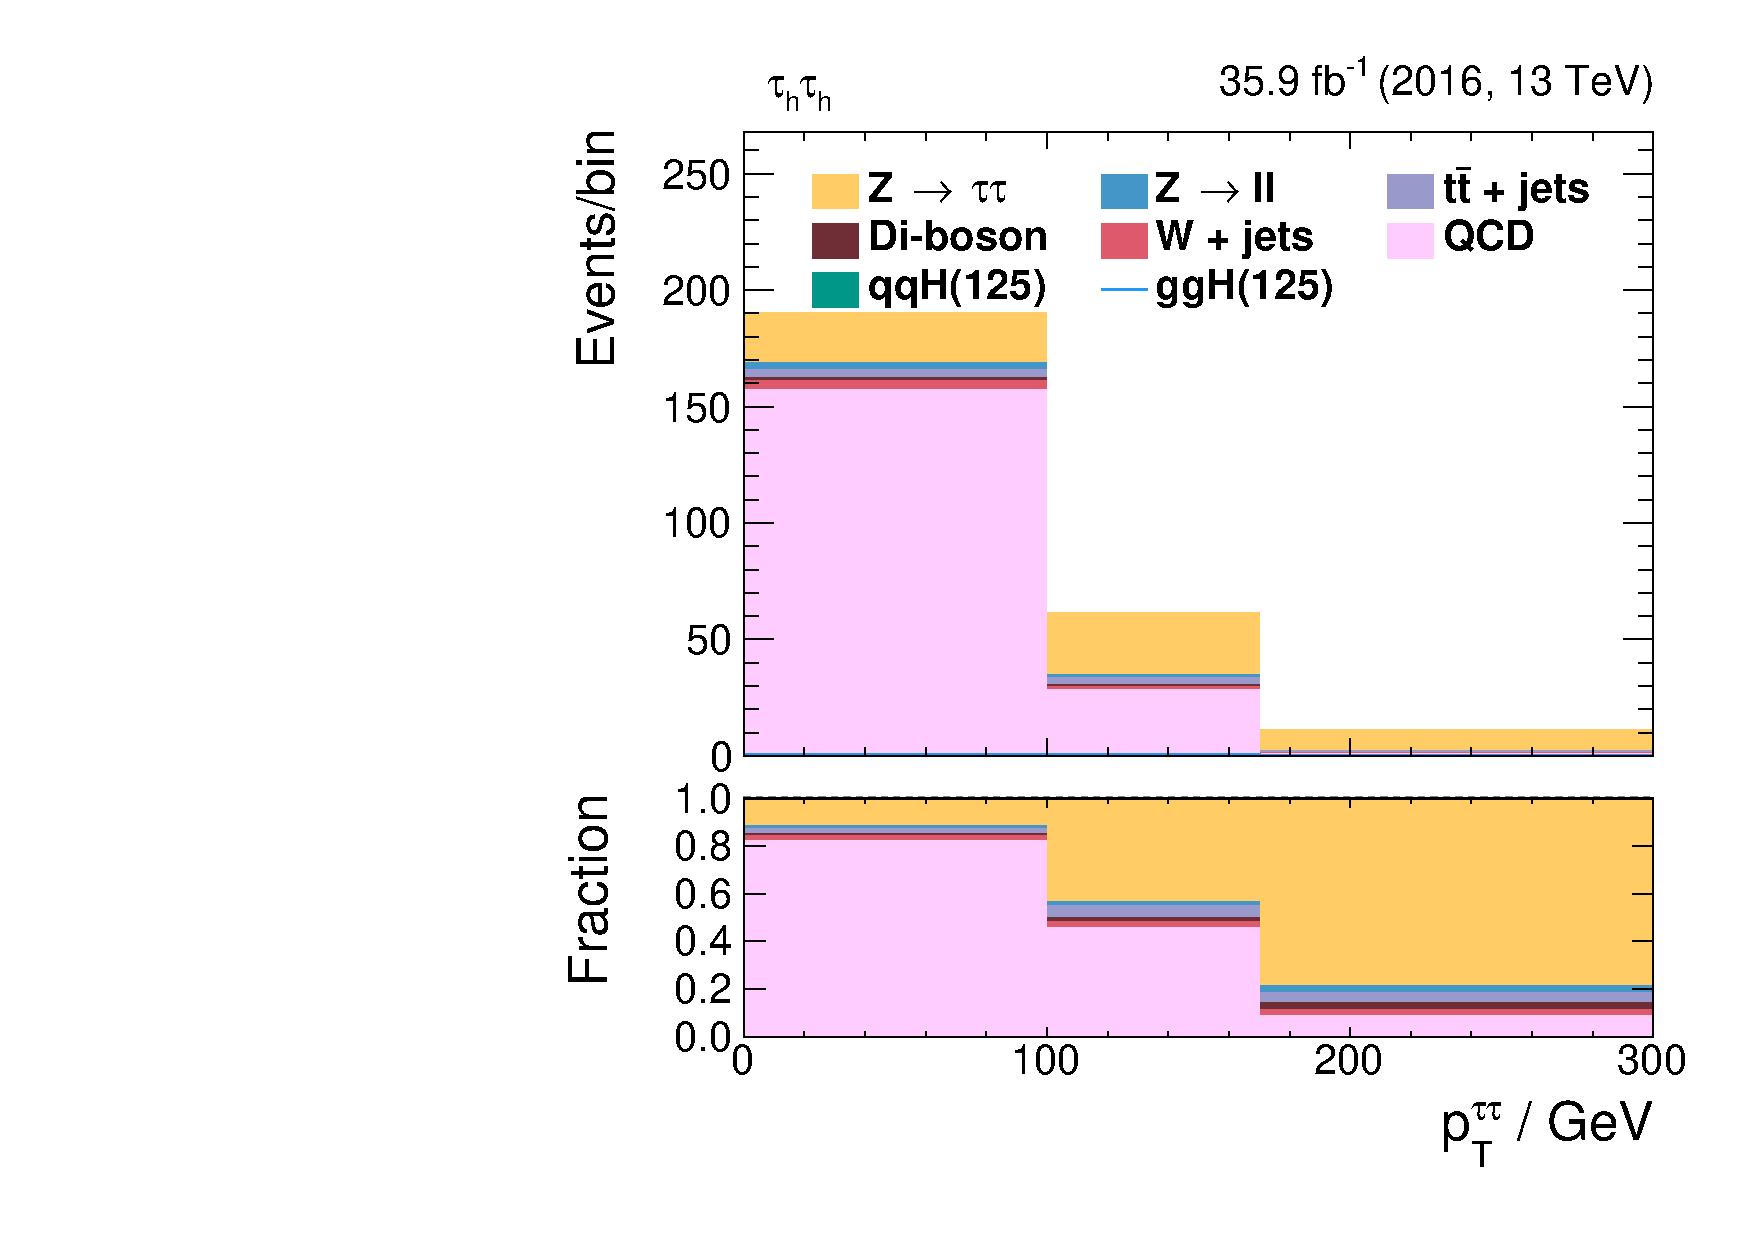
\includegraphics[width=\textwidth]{Figures/eventselection/tt/BoostedCP/H_pt.pdf}
    \end{subfigure} % 
    \caption[Background modeling in the \textit{0-jet} and \textit{boosted} categories.]{ Estimated background and ggF signal distributions of observables in the \textit{0-jet} category (left) and \textit{boosted} category (middle, right) for the $\tau_\text{h}\tau_\text{h}$ channel. 
    Background and signal are modeled from simulation. From the middle plot it can be inferred that the invariant ditau mass is capable of separating Higgs bosons from Drell-Yan background, as both the Z and the Higgs boson peaks are visible and separated. The subplot shows the relative fraction of each background in each bin. In the \tautau{} channel is the dominant background are multijet events. More plots can be found in the appendix \figref{SUPPLEMENT:ES:controlplots:0jet_boosted}.}\label{ES:controlplots:0jet_boosted}  
\end{figure}%

\subsubsection{Dijet signal categories}

Events containing two or more jets are further divided into a \textit{dijet boosted} and a \textit{dijet lowboost} category according to the
transverse momentum of the Higgs boson $p_\text{\,T}^{\tau\tau}$. 
To be part of the \textit{dijet boosted} category $p_\text{\,T}^{\tau\tau}>\text{200\,{GeV}}$ must be satisfied. Otherwise events fall in the \textit{lowboost} category.
As shown for the $\tau_\text{h}\tau_\text{h}$ channel in \figreft{ES:controlplots:0jet_boosted}, this criterion is particularly suited to separate signal from background.
Furthermore, the two jets in the dijet categories are required to have $m_\text{jj}>\text{300\,{GeV}}$ as discussed in \textreft{sec:jdphi} and \textreft{sec:jdphi}. The distribution of $m_\text{jj}$ for dijet events is shown in \figreft{ES:categorization:tt_distributions}.
In the final fit, three-dimensional  discriminators in bins of $m_{\tau\tau}$, $D_{0-}$, and $D_\text{CP}$ are constructed. The distributions of the individual observables and the background modeling are shown in \figreft{ES:controlplots:2jet_lowboost}. The categorization criteria are summarized in \tabreft{ES:categorization_2jet}. 
For the three observables the binnings
\begin{ct_version_list}
    \item $m_{\tau\tau} \in \left[ 0; 80;100;115;130;150;\infty \right]\text{\,{GeV}}$,
    \item $D_{0-} \in \left[ 0.0;0.25;0.5;0.75;1.0 \right]$, and
    \item $D_\text{CP} \in \left[ -1.0; -0.4;0.4;1.0 \right]$
\end{ct_version_list}%
were found to provide a reasonable compromise between sensitivity and bin population.
In principle two bins in $D_\text{CP}$ are sufficient to measure an asymmetry pointing to the presence of a CP violating term, but since it was observed that the event kinematics of different CP scenarios are rather similar, three bins were chosen.
The idea is that events with a clear signature, and therefore a high likelihood, found in the tails of the distribution get a larger impact on the analysis sensitivity.
The binning in $m_{\tau\tau}$ was chossen to find regions in the phase space with improved signal-to-background ratios close to the Higgs boson mass of $\text{125\,{GeV}}$.
% Distribution of mjj and Hpt to show that they can be used to reject background
% HiggsAnalysis/KITHiggsToTauTau/scripts/makePlots_controlPlots.py -i /nfs/dust/cms/user/dwolfsch/htautau/artus/2018-08-07_18-44_Run2CPStudies_Nominal_Summer16_plusHToTauTauM110-140/merged/ -s ztt zll ttj vv wj qcd qqh gghjhusm gghjhumm gghjhups -x mjj -c em et mt tt -w "(njets>1)" -a "  --live --formats pdf  --x-bins "50,0,2000" --scale-nicks gghjhumm125jhumm --scales 0.5 --y-log  --y-lims 0.1 100000"   --www EventSelection/Categorization --cpggh --background-method simeqn -n 4 --analysis-modules ScaleHistograms
% HiggsAnalysis/KITHiggsToTauTau/scripts/makePlots_controlPlots.py -i /nfs/dust/cms/user/dwolfsch/htautau/artus/2018-08-07_18-44_Run2CPStudies_Nominal_Summer16_plusHToTauTauM110-140/merged/ -s ztt zll ttj vv wj qcd qqh gghjhusm gghjhumm gghjhups -x H_pt -c em et mt tt -w "(njets>1)*(mjj>300)" -a "  --live --formats pdf --x-label \" p_{T}^{#tau#tau} / GeV \" --scale-nicks gghjhumm125_25jhumm --scales 0.5 --legend-cols 2 --legend 0.5 0.3 0.87 0.87  --x-bins "20,0,400" " --www EventSelection/Categorization --scale-signal 25 --cpggh --background-method simeqn --ratio-subplot --analysis-modules ScaleHistograms
% HiggsAnalysis/KITHiggsToTauTau/scripts/makePlots_controlPlots.py -i /nfs/dust/cms/user/dwolfsch/htautau/artus/2018-08-07_18-44_Run2CPStudies_Nominal_Summer16_plusHToTauTauM110-140/merged/ -s qqh gghjhusm gghjhumm gghjhups -x H_pt -c em et mt tt -w "(njets>1)*(mjj>300)" -a "  --live --formats pdf --x-label \" p_{T}^{#tau#tau} / GeV \" --filename H_pt_log --scale-nicks gghjhumm125jhumm --scales 0.5 --x-bins "20,0,400" " --www EventSelection/Categorization --cpggh --background-method simeqn --analysis-modules ScaleHistograms
\begin{figure}[h!]
    \centering
    \begin{subfigure}{.32\textwidth}
        \centering
        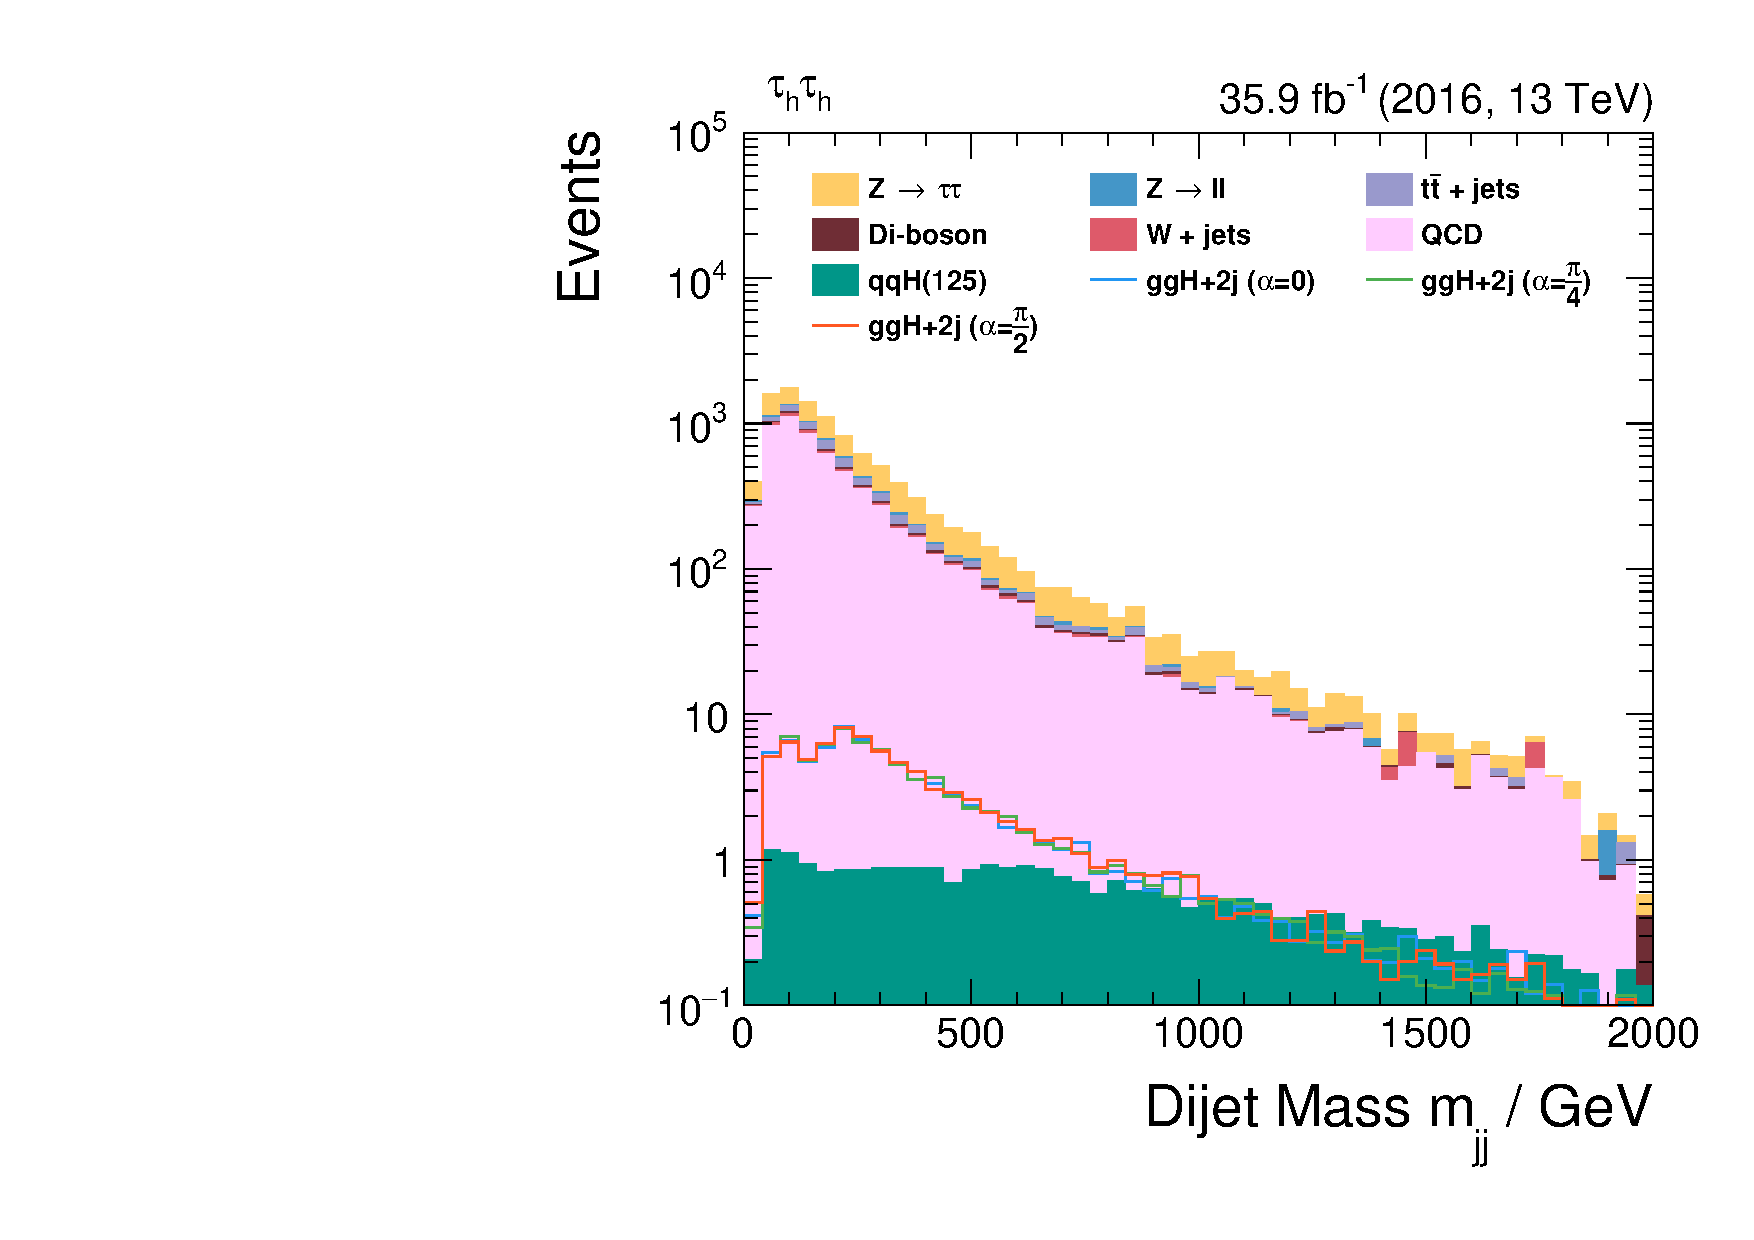
\includegraphics[width=\textwidth]{Figures/eventselection/Categorization/tt/mjj.pdf}
    \end{subfigure}%
    \begin{subfigure}{.32\textwidth}
        \centering
        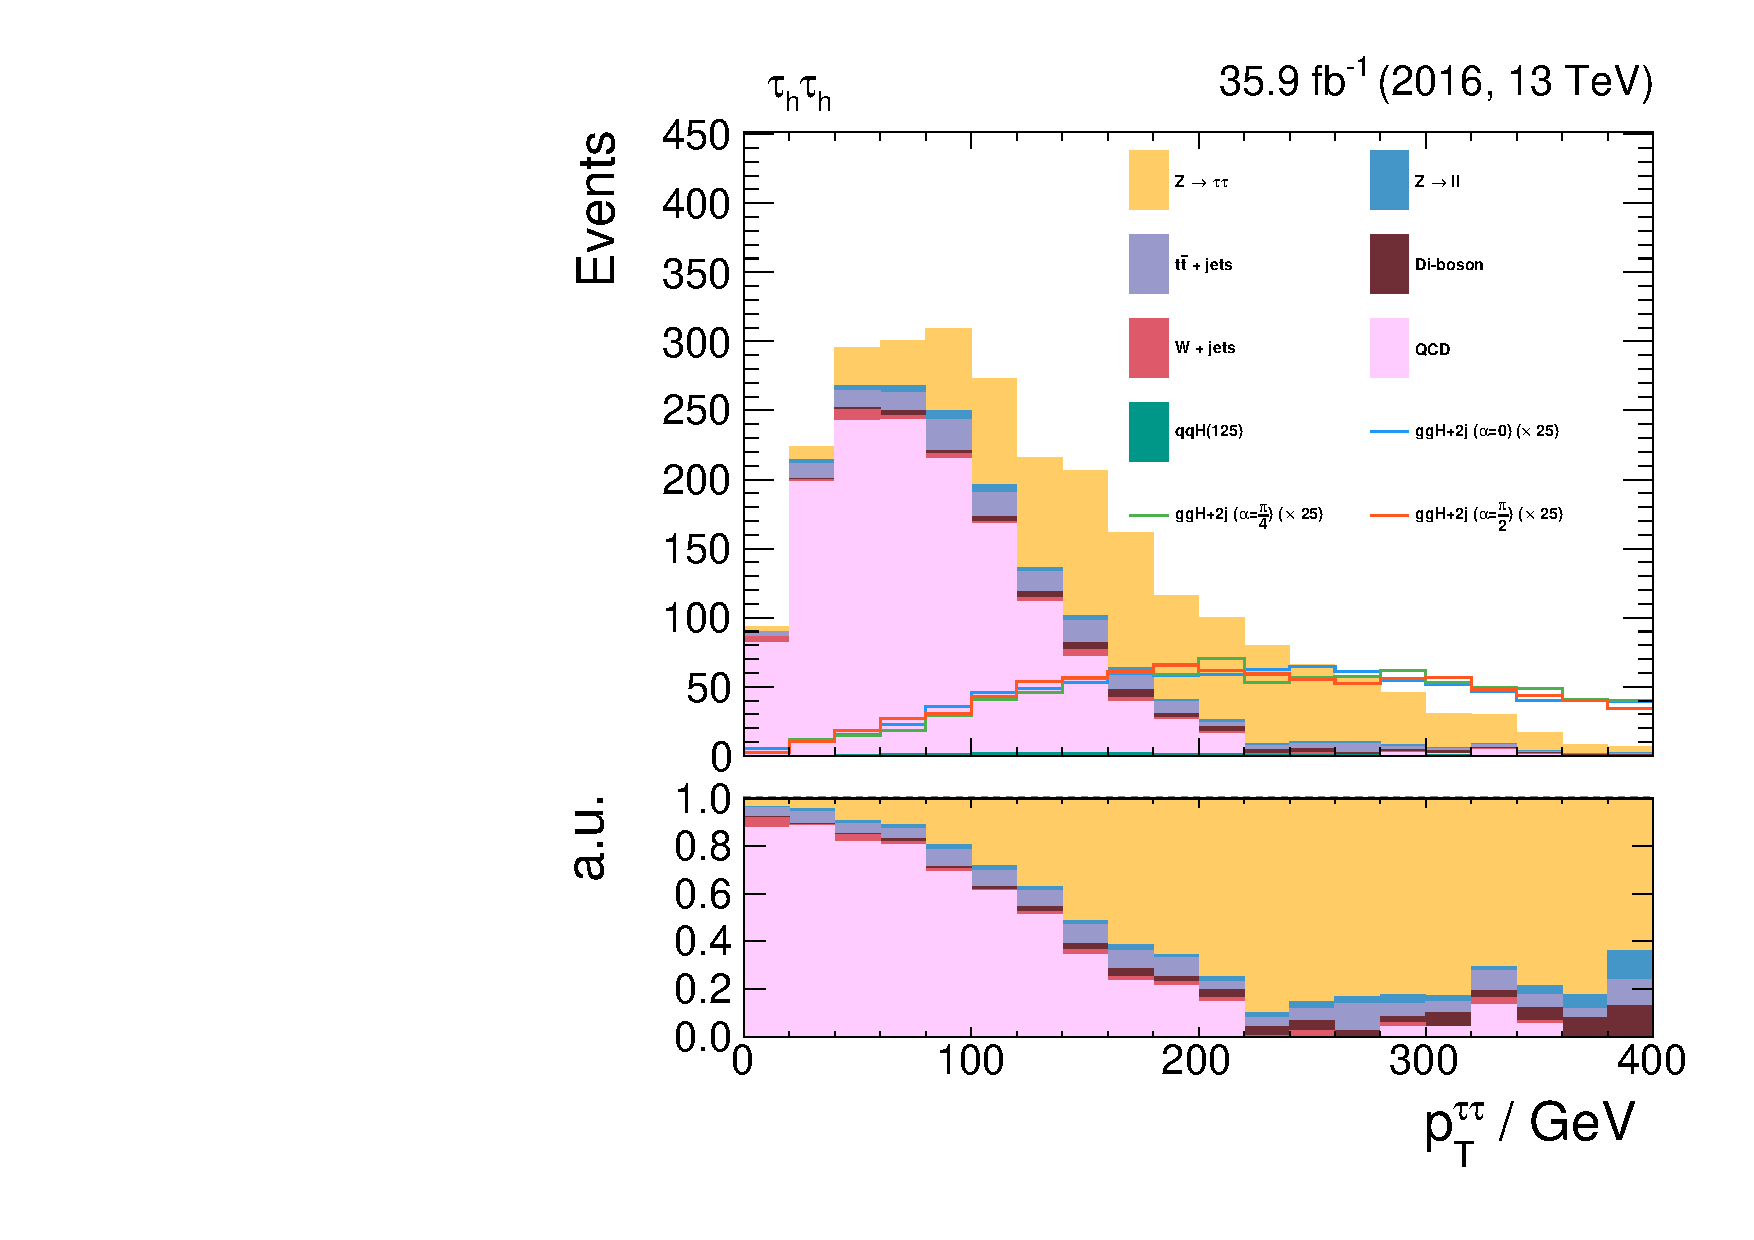
\includegraphics[width=\textwidth]{Figures/eventselection/Categorization/tt/H_pt.pdf}
    \end{subfigure}% 
    \begin{subfigure}{.32\textwidth}
        \centering
        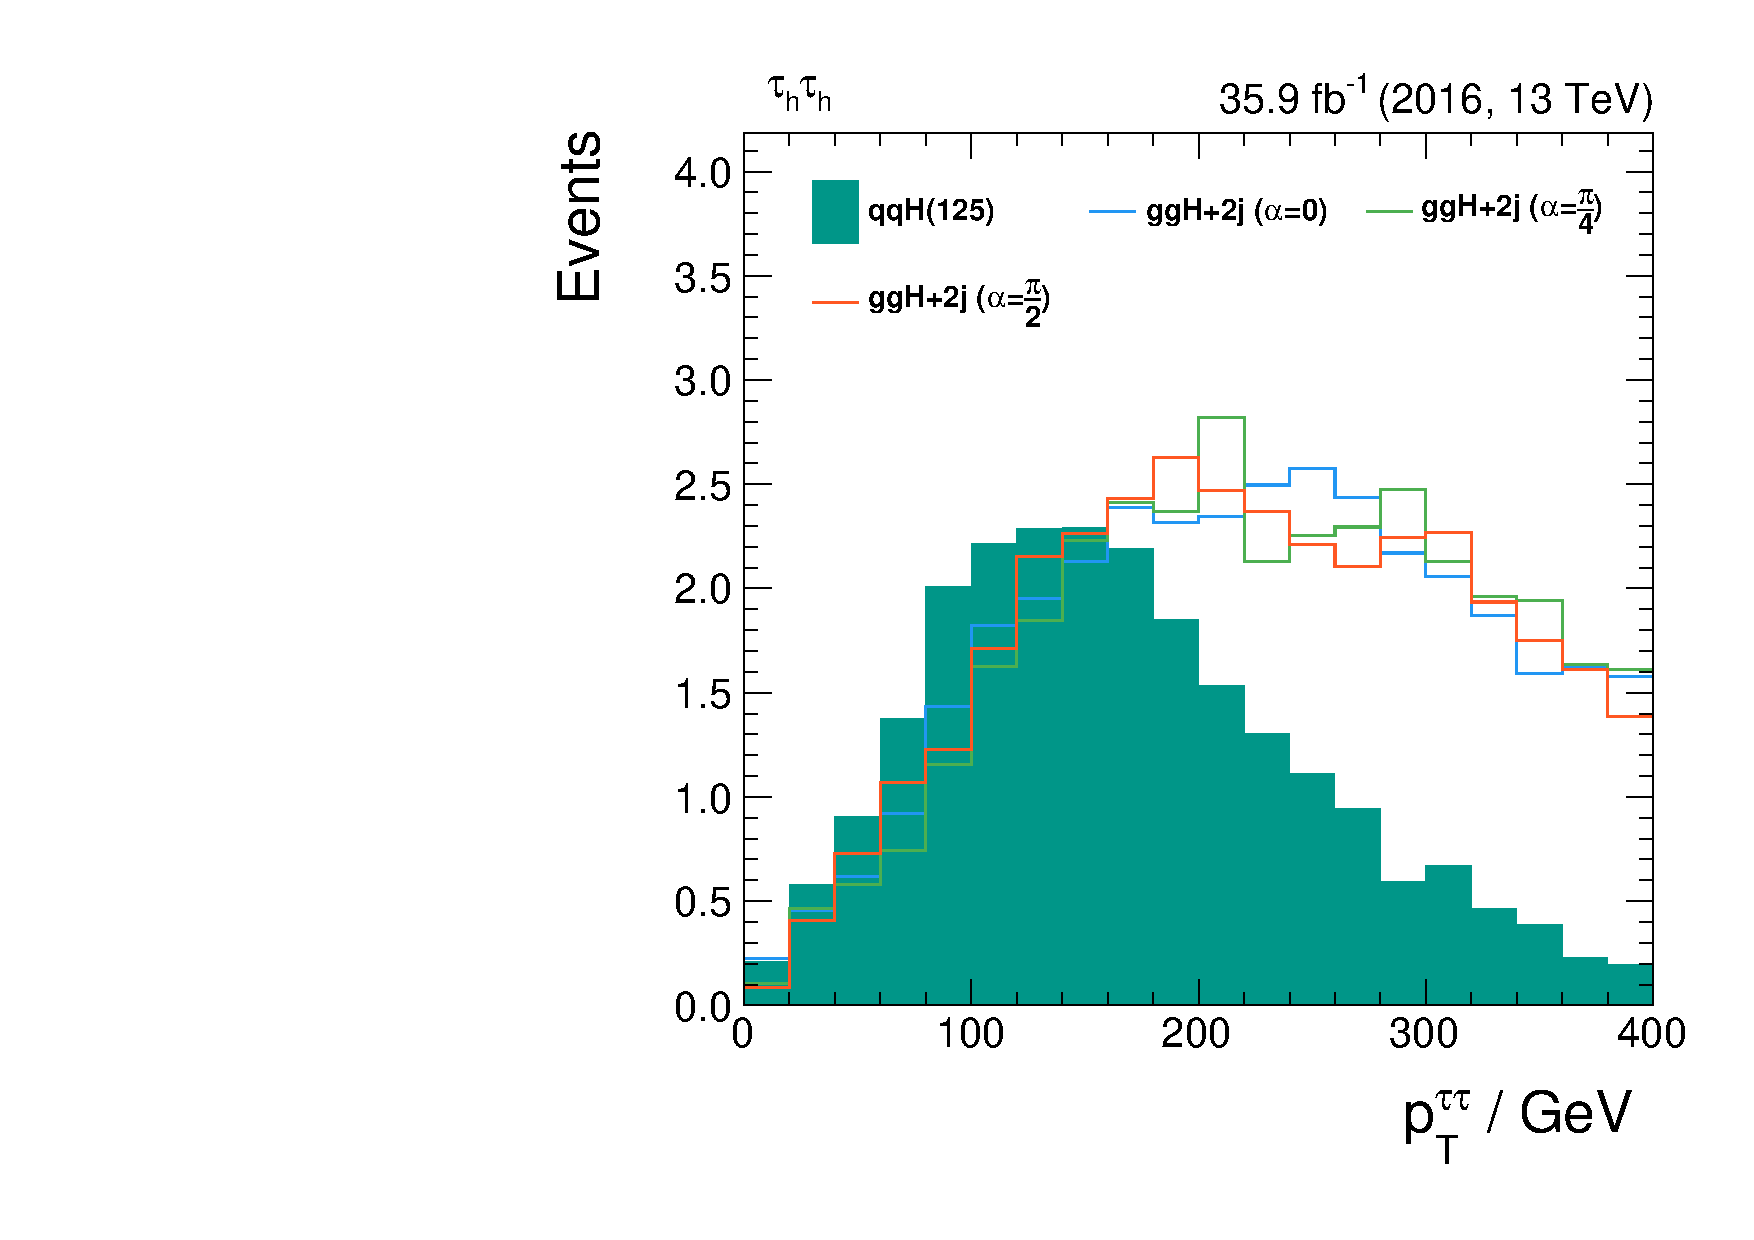
\includegraphics[width=\textwidth]{Figures/eventselection/Categorization/tt/H_pt_log.pdf}
    \end{subfigure}%     
    \caption[Background modeling in the \textit{dijet lowboost} and \textit{dijet boosted} categories.]{Expected signal and background modeling of the invariant dijet mass $m_\text{jj}$ (left) and the ditau transverse momentum $\vec{p}_{\text{T}}^{\tau\tau}$ (middle and right) for the $\tau_\text{h}\tau_\text{h}$ channel are shown for events with two jets or more. The cross section of all three CP scenarios are normalized to the SM ggF cross section. 
    The signal distributions in the middle plot of ditau transverse momentum is scaled by a factor of 25 for a better visibility.
    The right plots shows the same selection as applied in the middle plot focusing on the distributions of Higgs boson events. Above  $\vec{p}_{\text{T}}^{\tau\tau}=\text{200\,{GeV}}$ the fraction of ggF events compared to VBF events increases. More plots are shown \figreft{Supplement:ES:categorization:tt_distributions}.}\label{ES:categorization:tt_distributions}
\end{figure}

\begin{table}[!]
    \centering
    \caption[Dijet event categorization.]{Selection criteria and observables used in the two dijet categories.}\label{ES:categorization_2jet}
    \begin{tabular}{lllll}
        \toprule
        Channel         & dijet lowboost       & dijet boosted \\ \hline
        \multicolumn{3}{c}{Selection cuts}                       \\ \hline
        \multirow{2}{*}{$e\mu$}          & {\footnotesize >1 jet, $m_\text{jj}>\text{300\,{GeV}}$, $p_\text{\,T}^{\tau\tau}<\text{200\,{GeV}}$, }   &     {\footnotesize >1 jets, $m_\text{jj}>\text{300\,{GeV}}$, $p_\text{\,T}^{\tau\tau}>\text{200\,{GeV}}$, }           \\         
                                         & {\footnotesize $D_\zeta< \text{ -10\,{GeV}}$, \textit{b-tag veto} }                     &   {\footnotesize $D_\zeta< \text{ -10\,{GeV}}$, \textit{b-tag veto}  }  \\
        \multirow{2}{*}{$e\tau_\text{h}$}       & \multirow{2}{*}{{\footnotesize>1 jets, $ m_\text{jj}>\text{300\,{GeV}}$}}             &        \multirow{2}{*}{{\footnotesize >1 jets \& $ m_\text{jj}>\text{300\,{GeV}}$}  }      \\                
                                         &                                                                  &                                                               \\
        $\mu\tau_\text{h}$                      & {\footnotesize ,$p_\text{\,T}^{\tau\tau}<\text{200\,{GeV}}$, \textit{b-tag veto} }                       &          {\footnotesize$p_\text{\,T}^{\tau\tau}>\text{200\,{GeV}}$, \textit{b-tag veto}}      \\                
        $\tau_\text{h}\tau_\text{h}$  & {\footnotesize >1 jets, $m_\text{jj}>\text{300\,{GeV}}$, $p_\text{\,T}^{\tau\tau}<\text{200\,{GeV}}$ }                                            &      {\footnotesize >1 jets, $ m_\text{jj}>\text{300\,{GeV}}$, $p_\text{\,T}^{\tau\tau}>\text{200\,{GeV}}$  }          \\  \midrule 
        \multicolumn{3}{c}{Observables}                       \\ \hline
         All           &  \multicolumn{2}{c}{$m_{\tau\tau} \times D_\text{CP} \times D_{0-}$}  \\ \bottomrule                
    \end{tabular}%
\end{table}%

% Distribution of the observables in the dijet_lowboost and dijet-boosted categories
% makePlots_controlPlots.py -i /nfs/dust/cms/user/dwolfsch/htautau/artus/2018-08-07_18-44_Run2CPStudies_Nominal_Summer16_plusHToTauTauM110-140/merged/ -s ztt zll ttj vv wj qcd qqh gghjhusm gghjhumm gghjhups -x m_sv -c em et mt tt --categories dijet2D_lowboost dijet2D_boosted -a "  --live --formats pdf --scale-nicks gghjhumm125_10jhumm --scales 0.5  --x-bins \" 0.0 80.0 100.0 115.0 130.0 150.0 \" --y-label  \"dN/dm_{#tau #tau}(1/GeV)\" "  --scale-signal 10 --www EventSelection --cpggh --background-method simeqn --ratio-subplot --analysis-modules NormalizeByBinWidth ScaleHistograms -n 8
% makePlots_controlPlots.py -i /nfs/dust/cms/user/dwolfsch/htautau/artus/2018-08-07_18-44_Run2CPStudies_Nominal_Summer16_plusHToTauTauM110-140/merged/ -s ztt zll ttj vv wj qcd qqh gghjhusm gghjhumm gghjhups -x melaDiscriminatorD0MinusGGH -c em et mt tt --categories dijet2D_lowboost dijet2D_boosted -a " --live --formats pdf --scale-nicks gghjhumm125_10jhumm --scales 0.5  --x-bins \" 0.0 0.25 0.5 0.75 1.00 \" --y-label  \"dN/dD_{0-}^{ggH}\" " --scale-signal 10 --www EventSelection --cpggh --background-method simeqn --ratio-subplot --analysis-modules NormalizeByBinWidth ScaleHistograms -n 8
% makePlots_controlPlots.py -i /nfs/dust/cms/user/dwolfsch/htautau/artus/2018-08-07_18-44_Run2CPStudies_Nominal_Summer16_plusHToTauTauM110-140/merged/ -s ztt zll ttj vv wj qcd qqh gghjhusm gghjhumm gghjhups -x melaDiscriminatorDCPGGH -c em et mt tt --categories dijet2D_lowboost dijet2D_boosted -a " --live --formats pdf  --scale-nicks gghjhumm125_10jhumm --scales 0.5 --x-bins \" -1.0 -0.4 0.4 1.00 \" --y-label  \"dN/dD_{CP}^{ggH}\" " --scale-signal 10 --www EventSelection --cpggh --background-method simeqn --ratio-subplot --analysis-modules NormalizeByBinWidth ScaleHistograms -n 8

\begin{figure}[h!]
    \centering
    \begin{subfigure}{.32\textwidth}
        \centering
        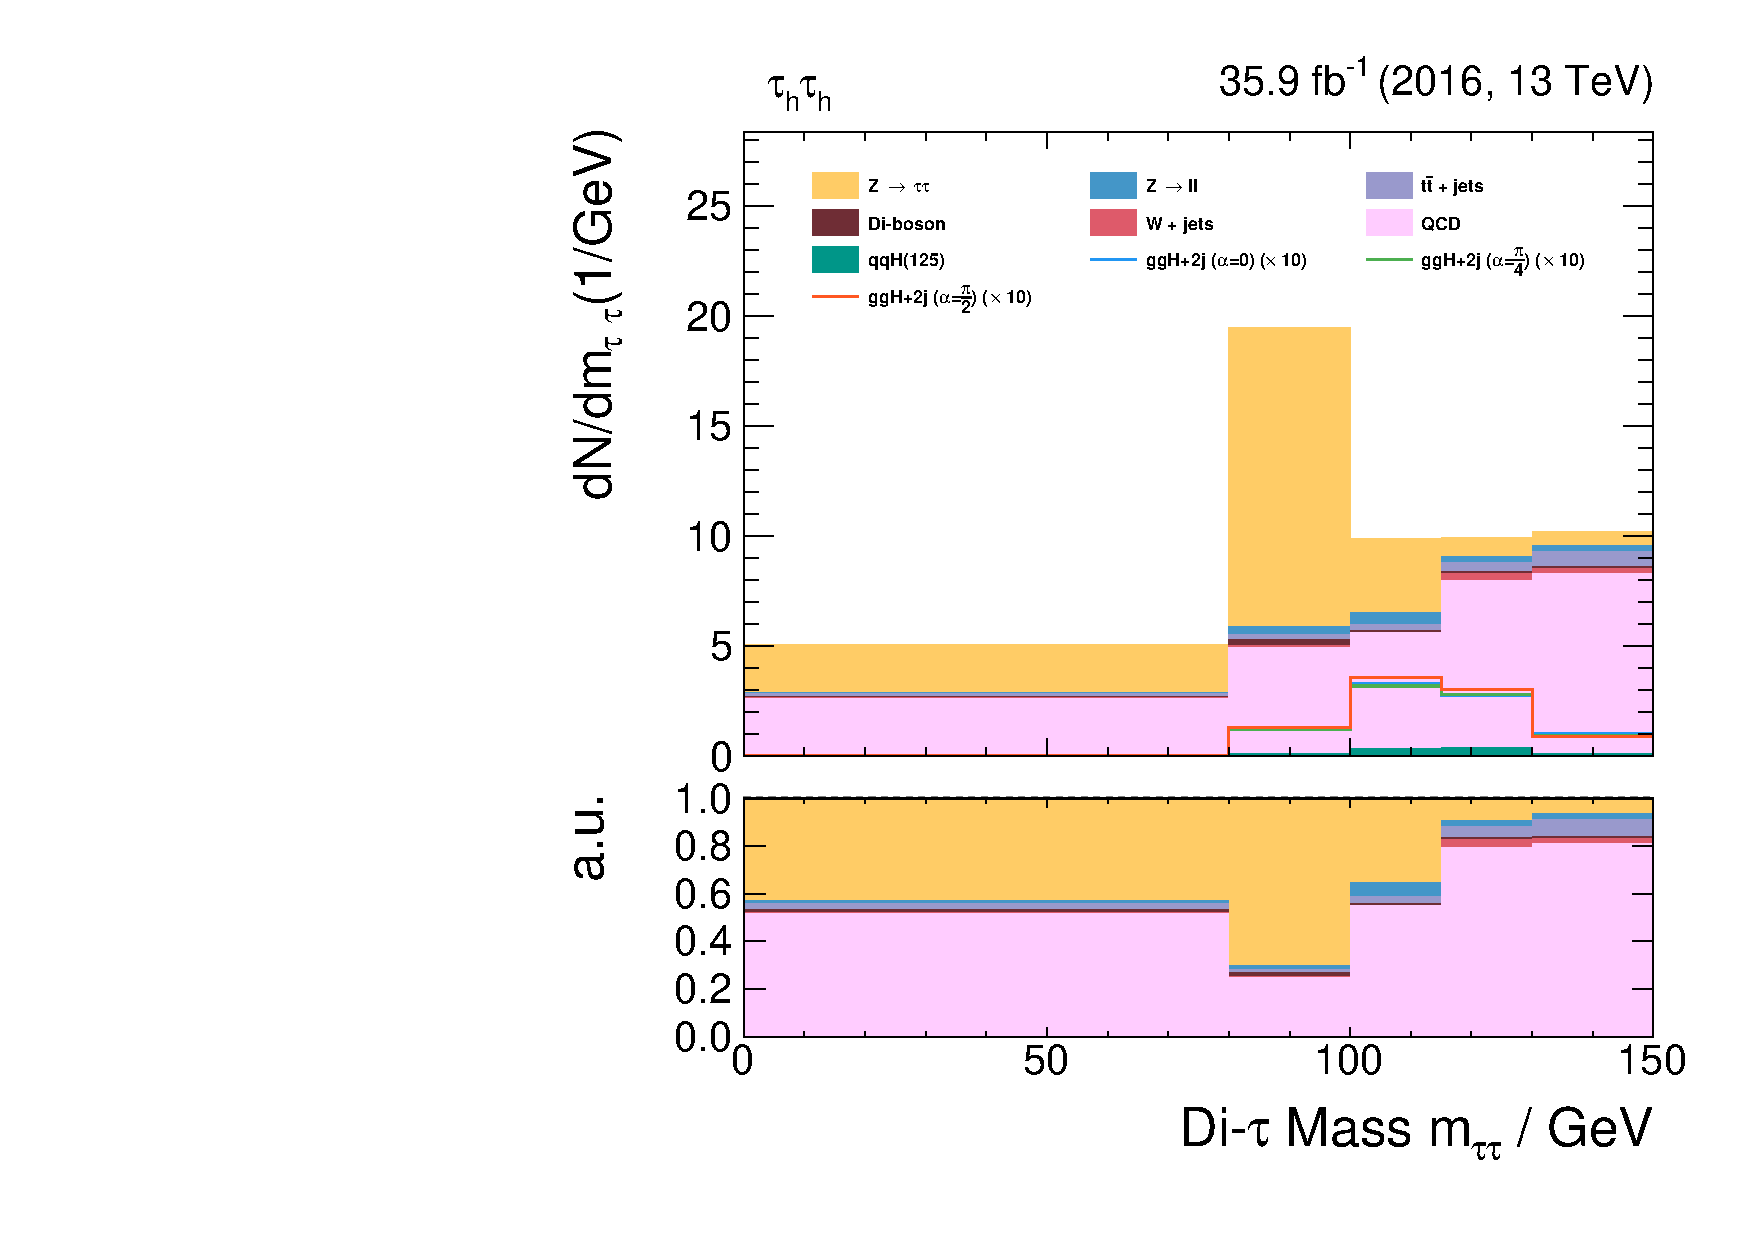
\includegraphics[width=\textwidth]{Figures/eventselection/tt/dijet2D_lowboost/m_sv.pdf}
    \end{subfigure}%
    \begin{subfigure}{.32\textwidth}
        \centering
        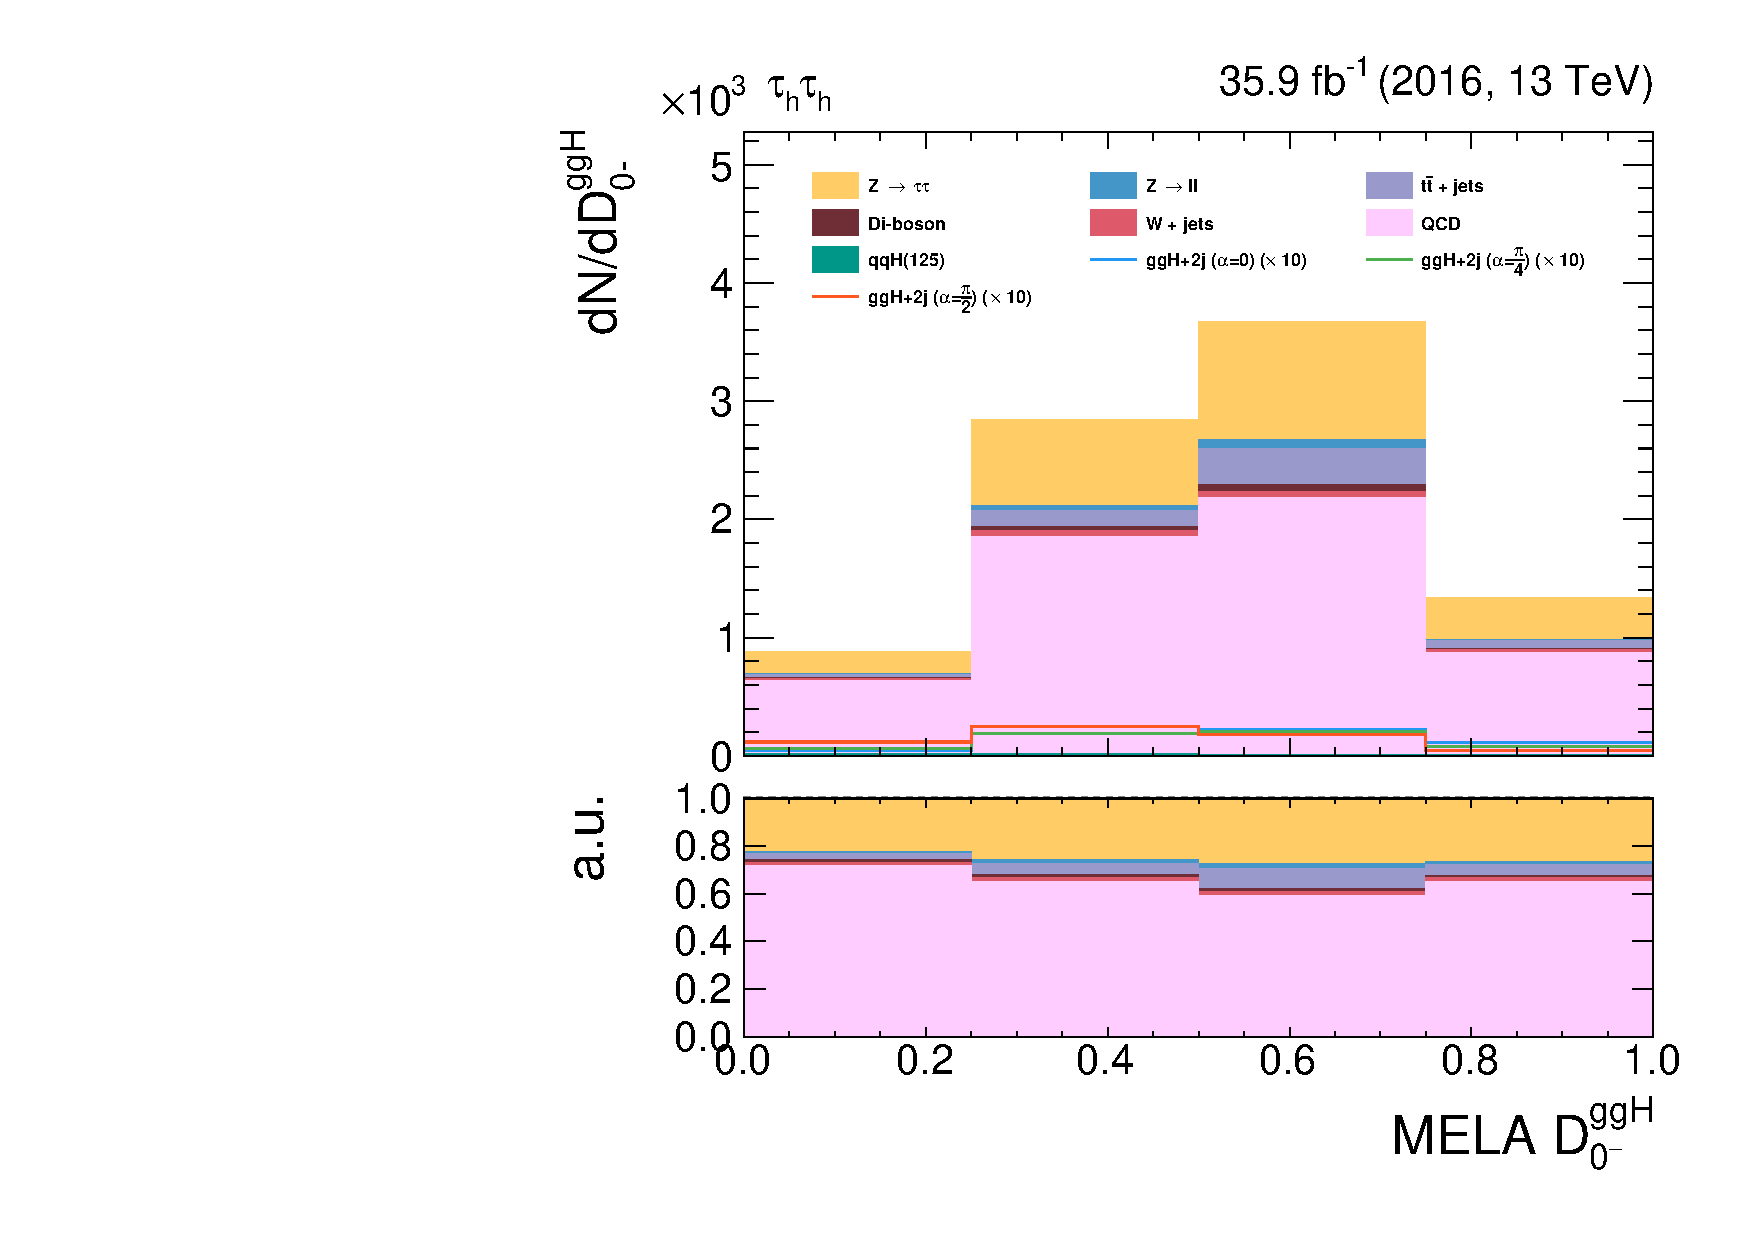
\includegraphics[width=\textwidth]{Figures/eventselection/tt/dijet2D_lowboost/melaDiscriminatorD0MinusGGH.pdf}
    \end{subfigure}%
    \begin{subfigure}{.32\textwidth}
        \centering
        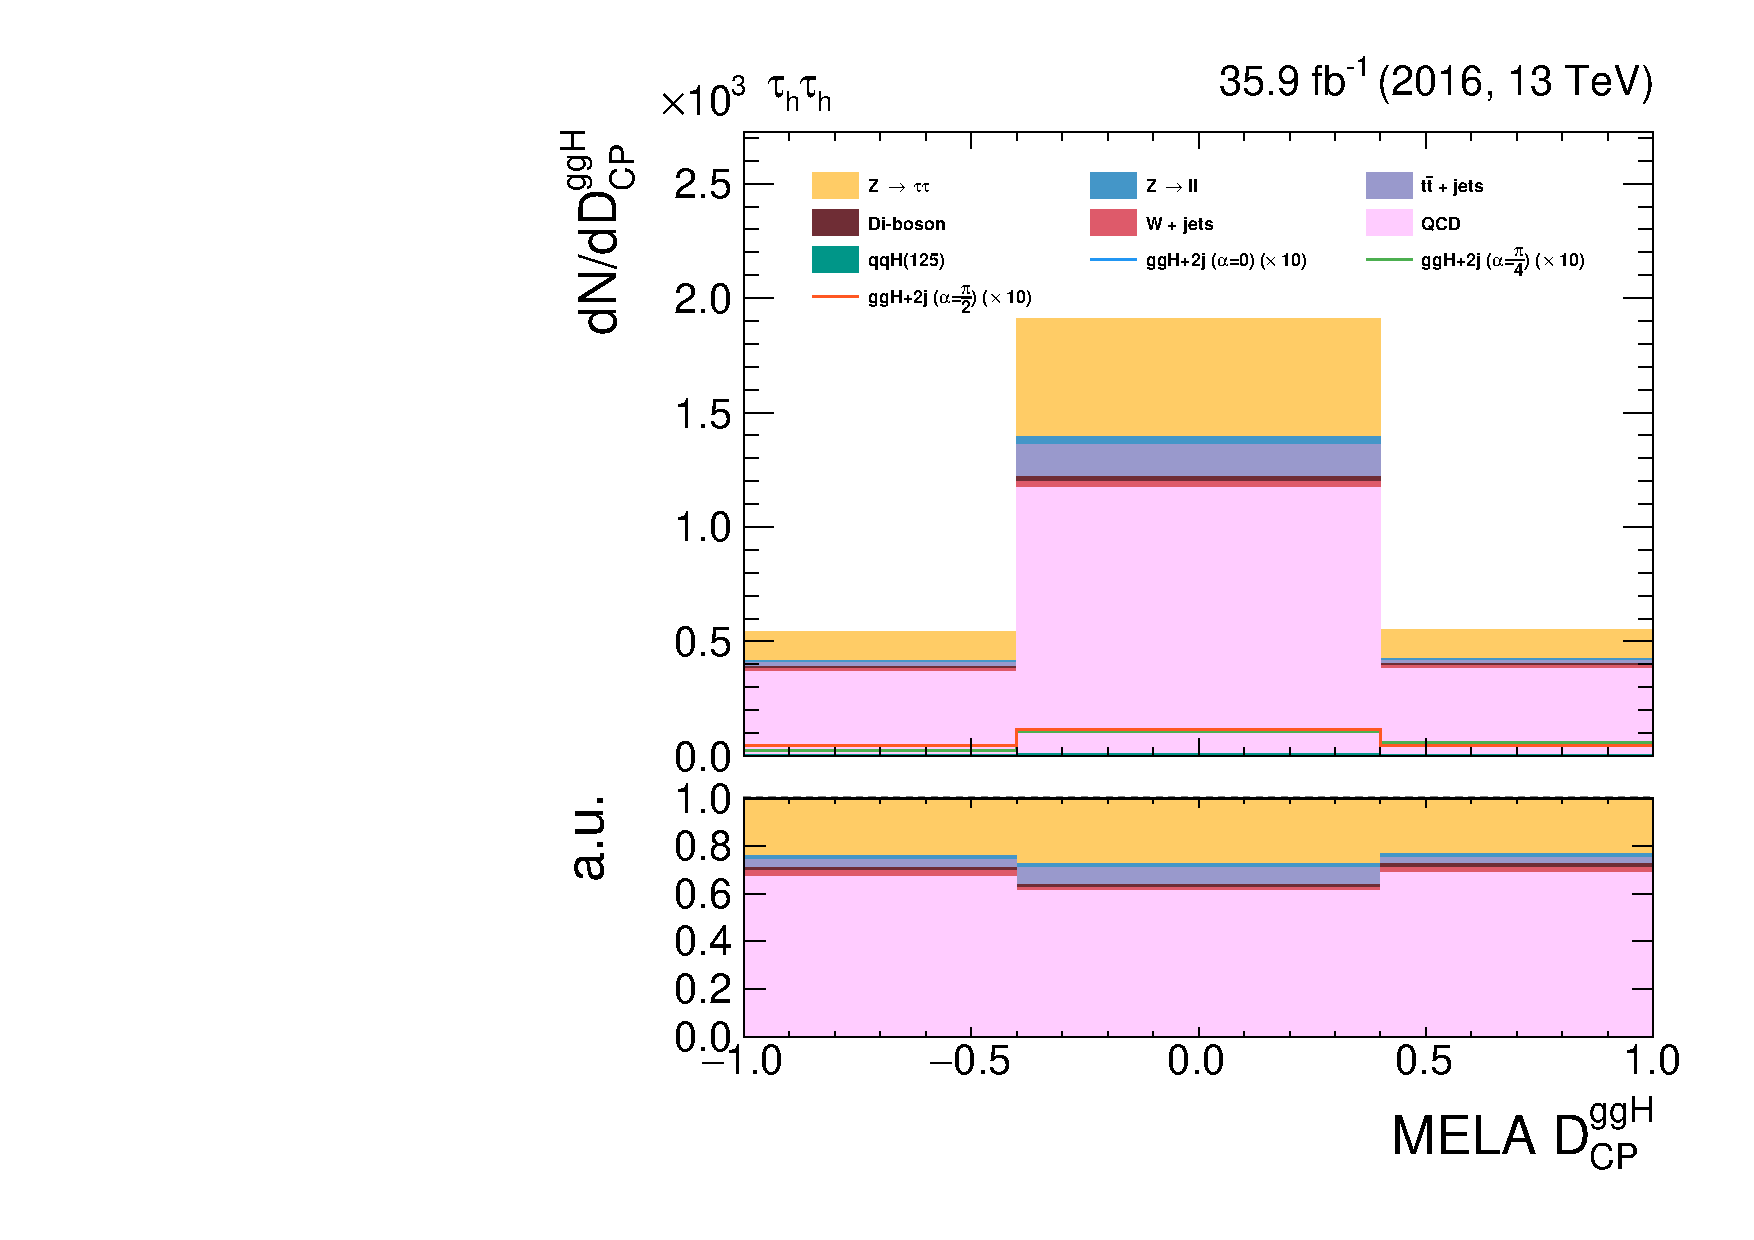
\includegraphics[width=\textwidth]{Figures/eventselection/tt/dijet2D_lowboost/melaDiscriminatorDCPGGH.pdf}
    \end{subfigure} % 
    \caption[\textit{Dijet lowboost} background modeling in the \tautau{} channel.]{Background and ggH signal distributions for a scalar (blue), a CP violating (green) and a pseudoscalar (orange) CP scenario of the observables in the dijet lowboost category for the $\tau_\text{h}\tau_\text{h}$ channel. 
    The cross section of the different CP scenarios are normalized to the SM ggF cross section.
    All histograms are normalized by the bin width and the ggF signal scaled by a factor 10 to improve the visibility. More plots can be found in \figreft{Supplement:ES:controlplots:2jet_lowboost}.}\label{ES:controlplots:2jet_lowboost}  
\end{figure}%

For cross-checks the analysis is also performed using $\Delta\phi_\text{jj}$ as a discriminating variable. In that approach a two-dimensional discriminator in bins of $m_{\tau\tau}$ and $\Delta\phi_\text{jj}$ is constructed. The binning 
used in this case is 
\begin{ct_version_list}
    \item  $m_{\tau\tau} \in \left[ 0; 80;100;115;130;150;\infty \right]\text{\,{GeV}}$ and
    \item  $\Delta\phi_\text{jj} \in \left[-3.2;-2.7;-2.1;-1.6;-1.1;-0.5;0.0;0.5;1.1;1.6;2.1;2.7;3.2 \right]$.
\end{ct_version_list}
As a qualitative test for the potential of the two CP sensitive observables to distinguish between different CP hypotheses the signal efficiency of a scalar Higgs boson coupling ($0^{++}$) is plotted versus the signal efficiency of a pseudoscalar Higgs boson coupling ($0^{-+}$).
This so-called \textit{ROC curve} is shown in \figreft{ES:ROC_curve} for the \textit{dijet boosted} category in the $\tau_\text{h}\tau_\text{h}$ channel. The curve proves the statement made before that the approach with the optimal observables
provides more potential than using $\Delta\phi_\text{jj}$ as a single observable. This means, there is indeed more spin information encapsulated in the remaining four angles that are fully taken into account by the matrix element likelihood approach.
% Command needed for ROC Curve - first to to get roc curve - third to plot in one plot.

 % higgsplot.py -i /nfs/dust/cms/user/dwolfsch/htautau/artus/2018-08-07_18-44_Run2CPStudies_Nominal_Summer16_plusHToTauTauM110-140/merged/GluGluH2JetsToTauTauM125CPmixingsmJHU_RunIISummer16MiniAODv2_PUMoriond17_13TeV_MINIAOD_JHUgen/GluGluH2JetsToTauTauM125CPmixingsmJHU_RunIISummer16MiniAODv2_PUMoriond17_13TeV_MINIAOD_JHUgen.root /nfs/dust/cms/user/dwolfsch/htautau/artus/2018-08-07_18-44_Run2CPStudies_Nominal_Summer16_plusHToTauTauM110-140/merged/GluGluH2JetsToTauTauM125CPmixingpseudoscalarJHU_RunIISummer16MiniAODv2_PUMoriond17_13TeV_MINIAOD_JHUgen/GluGluH2JetsToTauTauM125CPmixingpseudoscalarJHU_RunIISummer16MiniAODv2_PUMoriond17_13TeV_MINIAOD_JHUgen.root -f tt_nominal/ntuple -x "TMath::Sign(1,melaDiscriminatorDCPGGH)*melaDiscriminatorD0MinusGGH" --live --analysis-modules NormalizeToUnity CutEfficiency --nicks noplot_sm noplot_ps roc --cut-efficiency-sig-nicks noplot_ps --cut-efficiency-bkg-nicks noplot_sm --cut-efficiency-nicks roc --colors material_blue2 --x-bins "12,0,1" --plot-modules ExportRoot -w "(mjj>300)*(H_pt>200)*(njets>1)" --cut-efficiency-modes sigEffVsBkgEff --y-label "GF 0^{-+}" --x-label "GF 0^{++}" -o roc_curve --filename mela_roc  
 % higgsplot.py -i /nfs/dust/cms/user/dwolfsch/htautau/artus/2018-08-07_18-44_Run2CPStudies_Nominal_Summer16_plusHToTauTauM110-140/merged/GluGluH2JetsToTauTauM125CPmixingsmJHU_RunIISummer16MiniAODv2_PUMoriond17_13TeV_MINIAOD_JHUgen/GluGluH2JetsToTauTauM125CPmixingsmJHU_RunIISummer16MiniAODv2_PUMoriond17_13TeV_MINIAOD_JHUgen.root /nfs/dust/cms/user/dwolfsch/htautau/artus/2018-08-07_18-44_Run2CPStudies_Nominal_Summer16_plusHToTauTauM110-140/merged/GluGluH2JetsToTauTauM125CPmixingpseudoscalarJHU_RunIISummer16MiniAODv2_PUMoriond17_13TeV_MINIAOD_JHUgen/GluGluH2JetsToTauTauM125CPmixingpseudoscalarJHU_RunIISummer16MiniAODv2_PUMoriond17_13TeV_MINIAOD_JHUgen.root -f tt_nominal/ntuple -x "TMath::Abs(TMath::Sin(jdphi))" --live --analysis-modules NormalizeToUnity CutEfficiency --nicks noplot_sm noplot_ps roc --cut-efficiency-sig-nicks noplot_sm --cut-efficiency-bkg-nicks noplot_ps --cut-efficiency-nicks roc --colors material_blue2 --x-bins "20,0,1" --plot-modules ExportRoot -w "(mjj>300)*(H_pt>200)*(njets>1)" --cut-efficiency-modes sigEffVsBkgEff --y-label "GF 0^{-+}" --x-label "GF 0^{++}" -o roc_curve --filename sinjdphi_roc
% higgsplot.py -i roc_curve/sinjdphi_roc.root roc_curve/mela_roc.root -x roc --live --nicks jdphi mela --labels "sin(|#Delta#phi_{jj}|)" "D_{CP}*" --legend 0.2 0.75 0.45 0.92 --tree-draw-options TGraph -m L --colors material_blue2 material_orange --legend-markers L --x-label "ggH+2j(#alpha=0)" --y-label "ggH+2j(#alpha=#frac{#pi}{2})" --y-lims 0 1 --x-lims 0 1 --www roc_curve --filename ROC_curve --formats pdf --title "#tau_{h}#tau_{h}"

\begin{figure}[h!]
    \centering
    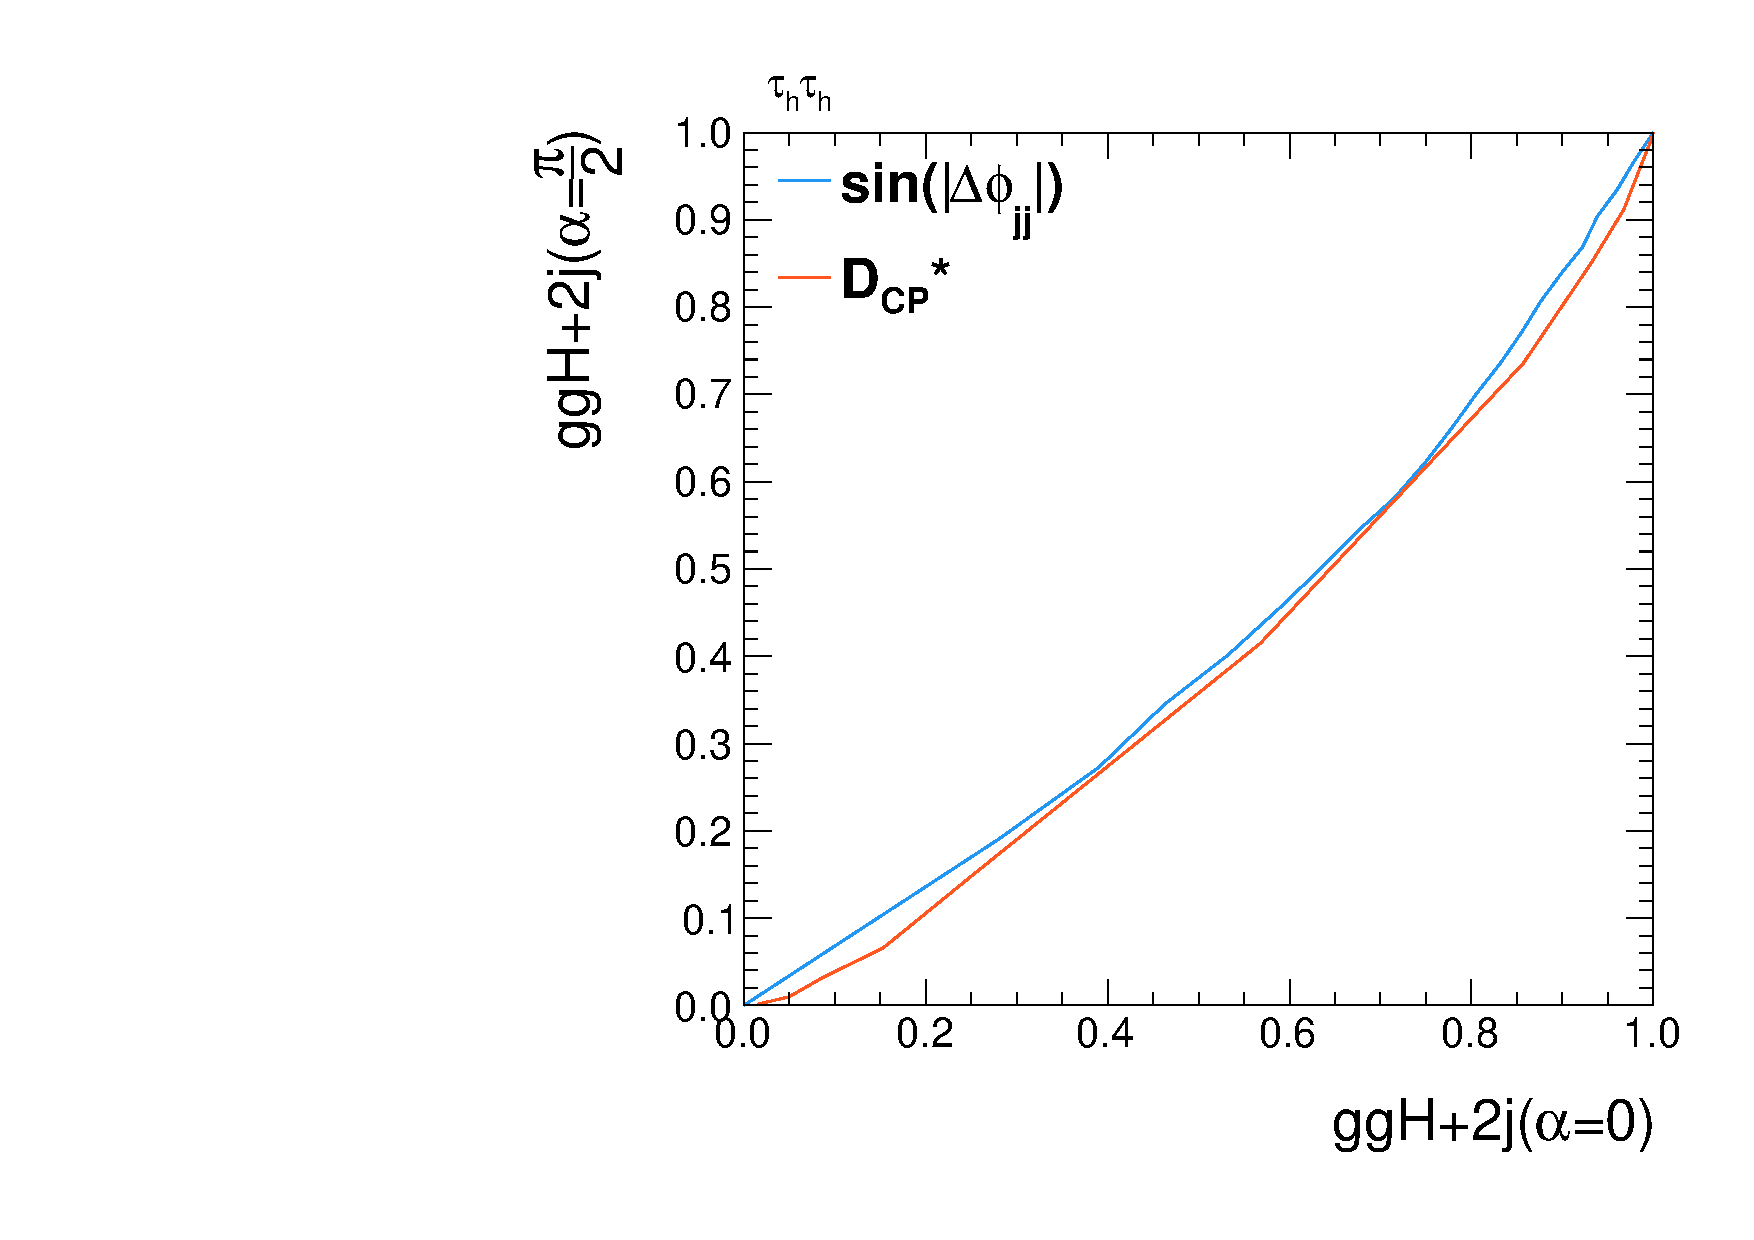
\includegraphics[width=.5\textwidth]{Figures/eventselection/ROC_curve}
    \caption[Distinguishability of kinematic and \jdphi{} approaches.]{Comparison of ability to separate scalar and pseudoscalar fermionic couplings in the $\tau_\text{h}\tau_\text{h}$ channel in the \textit{dijet boosted} category. 
    It can be seen, that the MELA approach has more potential to distinguish between scalar and pseudoscalar hypotheses.}\label{ES:ROC_curve}
\end{figure}%

\begin{table}[!]
    \centering
    \caption[Signal acceptances and background acceptances of the event categorization.]{Fraction in percent of ggF signal events (always first number given per cell), VBF background events (second number) and other background events (last number). The fractions are calcaluted from the
    histograms entering the final fit (Prefit). The categorization successfully provides the largest fraction of ggF events in the \textit{dijet boosted} category, where the fraction also superceeds the VBF contamination.}\label{ES:purities}
    \begin{tabular}{lcccc}
\toprule
\multicolumn{5}{c}{Fraction [\%] of ggF, VBF, Bkg events per channel and category}                         \\
 Channel/category &                 0-jet &               boosted &        dijet lowboost &         dijet boosted \\
\midrule
\multirow{2}{*}{$e\mu$   }                        &  0.29, 0.00,  &  0.51, 0.11,  &  0.85, 1.13,  &  4.74, 1.65, \\
                                                  &      99.71      &        99.38    &     98.01      &       93.61      \\   
\multirow{2}{*}{$e\tau_\text{h}$  }             &  0.47, 0.01,  &  0.67, 0.14,  &  0.81, 1.06,  &  4.66, 1.76, \\
                                                  &     99.53       &        99.20   &       98.13     &        93.58\     \\                
\multirow{2}{*}{$\mu\tau_\text{h}$ }            &  0.44, 0.01,  &  0.67, 0.13,  &  0.82, 1.15,  &  4.27, 1.76, \\
                                                  &     99.56       &        99.20   &      98.03      &        93.97     \\   
\multirow{2}{*}{$\tau_\text{h}\tau_\text{h}$} &  0.54, 0.01,  &  0.88, 0.20,  &  0.97, 1.22,  &  5.55, 2.11,  \\
                                                  &       99.45     &       98.92     &      97.81      &         92.34       \\   
\bottomrule
\end{tabular}

\end{table}%
\subsubsection{Purity and background contamination}
The fraction of ggF and VBF events per channel and category is calculated from the histograms corresponding to the one-dimensional, two-dimensional and three-dimensional discriminants that
are passed to the final fit. The contribution of VBF was split from the others backgrounds to cross-check whether indeed more ggF events than VBF events are selected.
As shown in \tabreft{ES:purities} the fraction of ggF is largest in the \textit{dijet boosted} category. Although VBF events tend to fall into the \textit{dijet boosted} category, too, they only superceed
ggF events in the \textit{dijet lowboost} category. This means that the \textit{lowboost} category is exceptionally capable of controlling the VBF background contamination in the final fit.\newline{}
Albeit the fraction of signal events does not exceed 6\% in any category, regions of phase space (especially bins of $m_{\tau\tau}$) can be found that show a larger signal-to-background ratio. These regions are produced by the combined binning of the three (two) discriminating observables
used in the matrix element ($\Delta\phi_\text{jj}$) approach.


\clearpage
